\section{Раздел 7: Нестандартные задачи}
Большинство задач решаются при помощи теории, изложенной выше.\\
1. Сколько чётных чисел в этом ряду: 16, 27, 258, 2667, 8888?\\
2. Сколько нечётных чисел в этом ряду: 16, 27, 258, 2667, 8888?\\
3. Какое самое маленькое чётное число можно составить из цифр 2, 4, 8 и 9, если каждую цифру надо использовать точно один раз?\\
4. Какое самое большое чётное число можно составить из цифр 2, 4, 8 и 9, если каждую цифру надо использовать точно один раз?\\
5. Расставьте скобки так, чтобы равенство было верным: $7\cdot9+12:3-2=23.$\\
6. Расставьте скобки так, чтобы равенство было верным: $20:2+7\cdot2-5=29.$

ewpage

oindent7. Разместите числа 1, 2, 3, 4, 5, 6, 7, 8, 9 в пустых кружках так, чтобы сумма трёх чисел расположенных на каждой прямой, была равна 15.
\begin{center}
\begin{figure}[h!]
\center{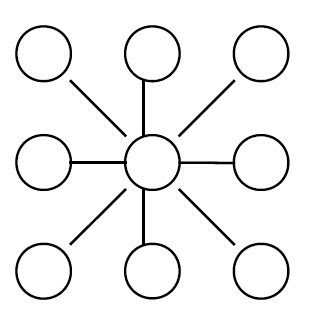
\includegraphics[scale=0.35]{2.png}}
\end{figure}
\end{center}
8. Разместите числа 2, 3, 4, 5, 6, 7, 8, 9, 10 в пустых кружках так, чтобы сумма трёх чисел расположенных на каждой прямой, была равна 18.
\begin{center}
\begin{figure}[h!]
\center{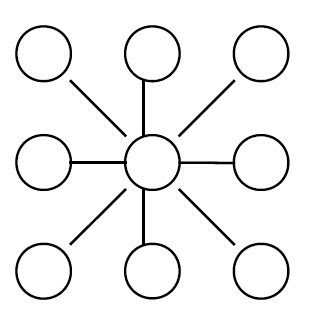
\includegraphics[scale=0.35]{22.png}}
\end{figure}
\end{center}
9. Назовём число {\it хорошим,} если его можно получить, перемножая только двойки и тройки. Перечислите все хорошие числа от 4 до 20.\\
10. Назовём число {\it хорошим,} если его можно получить, перемножая только двойки и пятёрки. Перечислите все хорошие числа от 6 до 30.\\
11. Представьте число 405 в виде произведения нескольких чисел, сумма которых равна 20.\\
12. Представьте число 575 в виде произведения нескольких чисел, сумма которых равна 37.\\
13. Имеются два кувшина: один объёмом 8 л, а второй --- объёмом 5 или 6 литров. На взгляд нельзя определить объём кувшина или воды в нём. Опишите, как определить объём второго кувшина, находясь возле реки.\\
14. Имеются два кувшина: один объёмом 5 л, а второй --- объёмом 3 или 4 литров. На взгляд нельзя определить объём кувшина или воды в нём. Опишите, как определить объём второго кувшина, находясь возле реки.\\
15. В шахматном турнире участвуют 14 человек. Сколько партий будет сыграно в турнире, если каждый участник сыграет со всеми остальными участниками по одному разу?\\
16. В чемпионате России по футболу участвуют 16 команд. Сколько матчей будет сыграно в чемпионате, если каждая команда сыграет со всеми остальными командами дважды?\\
17. Расположите в кружочках числа от 1 до 10 так, чтобы для любых двух соседних чисел их сумма была равна сумме двух чисел, им противоположных (симметричных относительно центра окружности).
\begin{center}
\begin{figure}[ht!]
\center{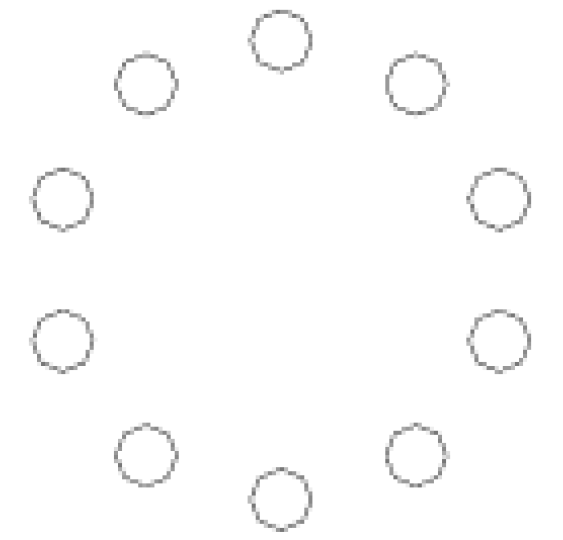
\includegraphics[scale=0.35]{3.png}}
\end{figure}
\end{center}

ewpage

oindent18. Расположите в кружочках числа от 11 до 20 так, чтобы для любых двух соседних чисел их сумма была равна сумме двух чисел, им противоположных (симметричных относительно центра окружности).
\begin{center}
\begin{figure}[ht!]
\center{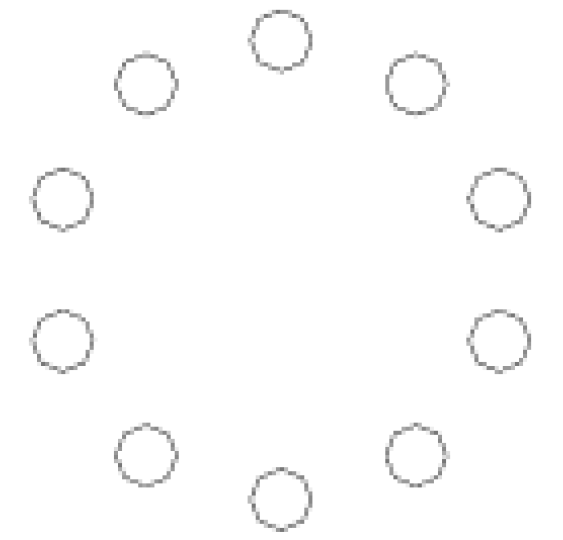
\includegraphics[scale=0.35]{33.png}}
\end{figure}
\end{center}
19. Сколько квадратов изображено на рисунке (все стороны маленьких квадратиков одинаковы)?
\begin{center}
\begin{figure}[ht!]
\center{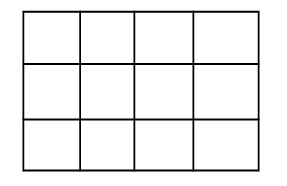
\includegraphics[scale=0.35]{4.png}}
\end{figure}
\end{center}
20. Сколько квадратов изображено на рисунке (все стороны маленьких квадратиков одинаковы)?
\begin{center}
\begin{figure}[ht!]
\center{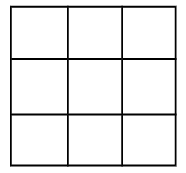
\includegraphics[scale=0.35]{44.png}}
\end{figure}
\end{center}
21. Сколько существует трёхзначных чисел, у которых все цифры чётные?\\
22. Сколько существует чётных трёхзначных чисел?\\
23. Какова разность между наибольшим и наименьшим четырёхзначными числами, все цифры которых различны?\\
24. Какова сумма наибольшего и наименьшего четырёхзначных чисел, все цифры которых различны?\\
25. Встретились три друга: Белов, Чернов и Рыжов. Один из них блондин, другой брюнет, а третий рыжий. Брюнет сказал Белову: <<Ни у кого из нас цвет волос не соответствует фамилии>>. Какой цвет волос у каждого из них?\\
26. В лесу проводился кросс. Белка сказала: <<Первое место занял заяц, а второй была лиса>>. Другая белка возразила: <<Заяц занял второе место, а лось был первым>>. На что филин заметил, что в высказывании каждой белки одна часть верная, а другая нет. Кто был первым, а кто вторым в кроссе?\\
27. Расставьте между цифрами знаки действий и скобки так, чтобы получилось верное равенство:\\ 5 4 3 2 1 = 100.\\
28. Расставьте между цифрами знаки действий и скобки так, чтобы получилось верное равенство:\\ 6 8 20 4 2 = 58.\\
29. Петя ходит в бассейн один раз в два дня, Коля --- один раз в 4 дня, а Вова --- один раз в пять дней. Они встретились в бассейне во вторник. В какой день недели они встретятся вновь?\\
30. Марина ходит в спортзал один раз в 6 дней, Маша --- один раз в 3 дня, а Катя --- один раз в 4 дня. Они встретились в спортзале в субботу. В какой день недели они встретятся вновь?

ewpage

oindent31. Расставьте в клетках данной таблицы числа 4, 5, 6, 7, 8, 9, 10, 11, 12 (по одному каждое) так, чтобы сумма чисел в каждой строке, каждом столбце и на двух главных диагоналях была равна 24.
\begin{center}
\begin{figure}[ht!]
\center{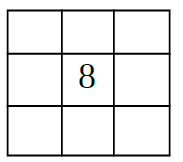
\includegraphics[scale=0.35]{5.png}}
\end{figure}
\end{center}
32. Расставьте в клетках данной таблицы числа 0, 1, 2, 3, 4, 5, 6, 7, 8 (по одному каждое) так, чтобы сумма чисел в каждой строке, каждом столбце и на двух главных диагоналях была одинаковой.
\begin{center}
\begin{figure}[ht!]
\center{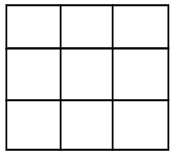
\includegraphics[scale=0.35]{55.png}}
\end{figure}
\end{center}
33. На какую цифру оканчивается сумма $9\times19\times29\times\ldots\times20129+1?$\\
34. На какую цифру оканчивается разность $4\times14\times24\times\ldots\times20124-1?$\\
35. Сколько существует пятизначных чисел, у которых третья цифра 7, а последняя цифра чётная?\\
36. Сколько различных трёхзначных чисел, меньших 400, можно составить из цифр 1, 3, 5, 7, 9, если любая из этих цифр может быть использована только один раз?\\
37. В числе 3728106 зачеркните 3 цифры так, чтобы оставшиеся цифры (в той же последовательности) образовывали:\\
а) возможно большее четырёхзначное число;\\
б) возможно меньшее четырёхзначное число.\\
38. В числе 4791402 зачеркните 3 цифры так, чтобы оставшиеся цифры (в той же последовательности) образовывали:\\
а) возможно большее четырёхзначное число;\\
б) возможно меньшее четырёхзначное число.\\
39. Сколькими способами можно расставить на полке томики стихов Пушкина, Лермонтова, Некрасова, Маршака и Барто, чтобы Пушкин стоял на первом месте, а Маршак и Барто стояли рядом?\\
40. Сколькими способами можно расставить на полке томики сказок Пушкина, Андерсена, Перро, Бажова и Гримм, чтобы Пушкин стоял на первом месте, а Бажов и Андерсен стояли рядом?\\
41. Перед вами МНОГОУГОЛЬНИК. У него может быть сколько угодно ВЕРШИН. ({\it На предложенном рисунке их всего 6, для примера.}) Представьте себе двадцатиугольник (у него 20 вершин). Одну из его вершин соединим отрезками со всеми остальными. На сколько треугольников мы разделим двадцатиугольник?
\begin{center}
\begin{figure}[ht!]
\center{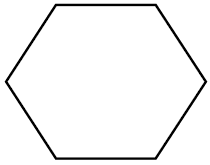
\includegraphics[scale=0.35]{6.png}}
\end{figure}
\end{center}
42. Перед вами МНОГОУГОЛЬНИК. У него может быть сколько угодно ВЕРШИН. ({\it На предложенном рисунке их всего 6, для примера.}) Представьте себе тридцатиугольник (у него 30 вершин). Одну из его вершин соединим отрезками со всеми остальными. На сколько треугольников мы разделим тридцатиугольник?
\begin{center}
\begin{figure}[ht!]
\center{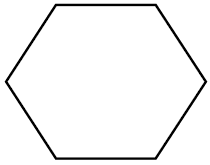
\includegraphics[scale=0.35]{6.png}}
\end{figure}
\end{center}

ewpage

oindent43. В клетках квадрата $3\times3$ были записаны натуральные числа так, что суммы в каждой строке, в каждом столбце и на каждой диагонали были одинаковыми. Некоторые числа стёрли. Восстановите стёртые числа.
\begin{center}
\begin{figure}[ht!]
\center{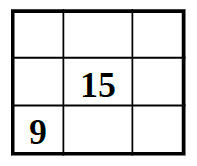
\includegraphics[scale=0.35]{7.png}}
\end{figure}
\end{center}
44. В клетках квадрата $3\times3$ были записаны натуральные числа так, что суммы в каждой строке, в каждом столбце и на каждой диагонали были одинаковыми. Некоторые числа стёрли. Восстановите стёртые числа.
\begin{center}
\begin{figure}[ht!]
\center{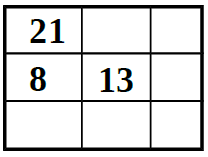
\includegraphics[scale=0.35]{77.png}}
\end{figure}
\end{center}
45. Расставьте четыре нечётных числа, среди которых нет равных, в квадраты так, чтобы их сумма равнялась 50.
\begin{center}
\begin{figure}[ht!]
\center{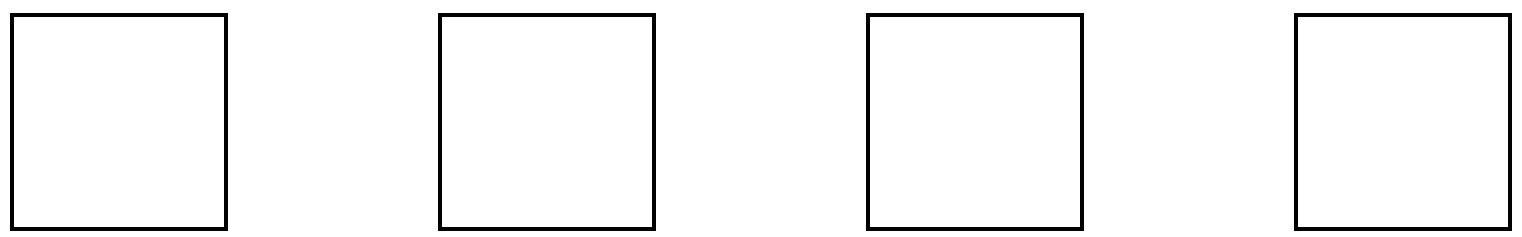
\includegraphics[scale=0.35]{8.png}}
\end{figure}
\end{center}
46. Расставьте четыре нечётных числа, среди которых нет равных, в квадраты так, чтобы их сумма равнялась 56.
\begin{center}
\begin{figure}[ht!]
\center{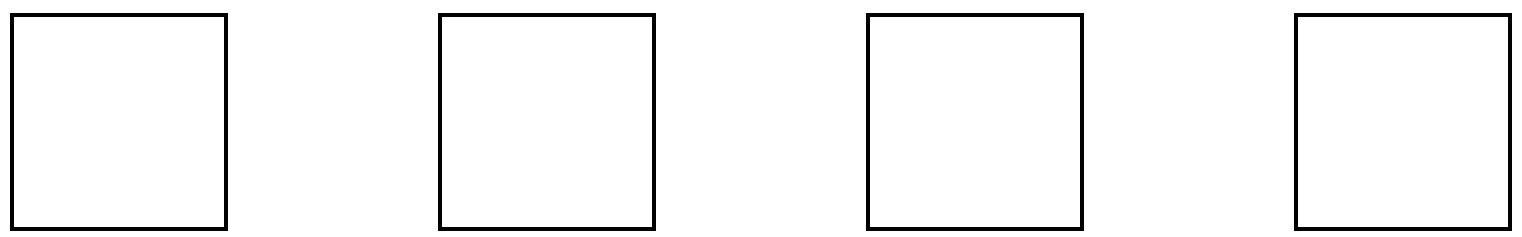
\includegraphics[scale=0.35]{8.png}}
\end{figure}
\end{center}
47. Придумайте пять различных чисел с суммой 120 таких, что любые два из них отличаются не более, чем на 4. В ответ запишите пять чисел через запятую.\\
48. Придумайте пять различных чисел с суммой 110 таких, что любые два из них отличаются не более, чем на 4. В ответ запишите пять чисел через запятую.\\
49. Сколько существует стозначных чисел, сумма цифр которых равна 16, у которых в разряде десятков стоит 2, в разряде сотен --- 3, а в разряде миллиардов --- 9?\\
50. Сколько существует девяностозначных чисел, сумма цифр которых равна 17, у которых в разряде сотен стоит 2, в разряде тысяч --- 4, а в разряде миллионов --- 9?\\
51. На рисунке изображена буква {\bf Т} ширины 7, высоты 6, а толщина ножки и шляпки у неё 3 клетки. Сколько клеток содержит аналогичная буква {\bf Т} ширины 70, высоты 60 и толщиной ножки и шляпки 6 клеток?
\begin{center}
\begin{figure}[ht!]
\center{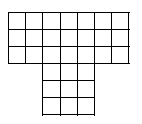
\includegraphics[scale=0.35]{9.png}}
\end{figure}
\end{center}

ewpage

oindent52. На рисунке изображена буква {\bf Т} ширины 7, высоты 6, а толщина ножки и шляпки у неё 3 клетки. Сколько клеток содержит аналогичная буква {\bf Т} ширины 60, высоты 70 и толщиной ножки и шляпки 8 клеток?
\begin{center}
\begin{figure}[ht!]
\center{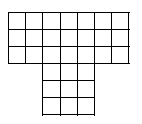
\includegraphics[scale=0.35]{9.png}}
\end{figure}
\end{center}
53. На рисунке изображена буква {\bf П} ширины 7, высоты 5, а толщина ножек и перекладины у неё 2 клетки. Сколько клеток содержит аналогичная буква {\bf П} ширины 70, высоты 60 и с толщиной ножки и перекладины 6 клеток?
\begin{center}
\begin{figure}[ht!]
\center{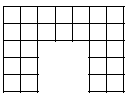
\includegraphics[scale=0.35]{10.png}}
\end{figure}
\end{center}
54. На рисунке изображена буква {\bf П} ширины 7, высоты 5, а толщина ножек и перекладины у неё 2 клетки. Сколько клеток содержит аналогичная буква {\bf П} ширины 60, высоты 80 и с толщиной ножки и перекладины 7 клеток?
\begin{center}
\begin{figure}[ht!]
\center{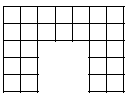
\includegraphics[scale=0.35]{10.png}}
\end{figure}
\end{center}
55. Придумайте пять различных двузначных нечётных чисел с суммой 375. В ответ запишите пять чисел через запятую.\\
56. Придумайте пять различных двузначных нечётных чисел с суммой 115. В ответ запишите пять чисел через запятую.\\
57. Расставьте цифры от 1 до 9 (каждую по одному разу) в квадратики так, чтобы все равенства были верными.
\begin{center}
\begin{figure}[ht!]
\center{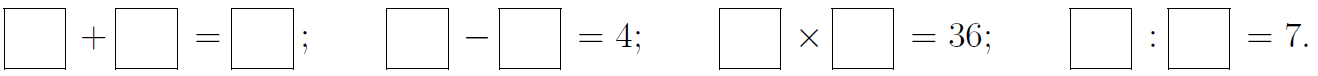
\includegraphics[scale=0.35]{11.png}}
\end{figure}
\end{center}
58. Расставьте цифры от 1 до 9 (каждую по одному разу) в квадратики так, чтобы все равенства были верными.
\begin{center}
\begin{figure}[ht!]
\center{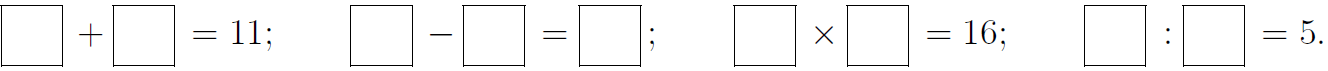
\includegraphics[scale=0.35]{111.png}}
\end{figure}
\end{center}
59. Сколько есть способов вычеркнуть несколько цифр из числа 56115664783047830888 так, чтобы осталось число 478?\\
60. Сколько есть способов вычеркнуть несколько цифр из числа 32111235692056920999 так, чтобы осталось число 569?\\
61. Суммарная длина перегородок в клетчатом прямоугольнике $4\times5$ на рисунке равна 31. Чему равна суммарная длина перегородок в прямоугольнике $12\times50?$
\begin{center}
\begin{figure}[ht!]
\center{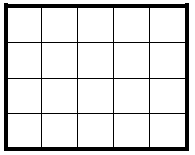
\includegraphics[scale=0.35]{12.png}}
\end{figure}
\end{center}

ewpage

oindent62. Суммарная длина перегородок в клетчатом прямоугольнике $4\times5$ на рисунке равна 31. Чему равна суммарная длина перегородок в прямоугольнике $40\times15?$
\begin{center}
\begin{figure}[ht!]
\center{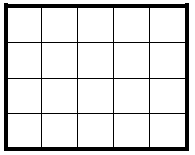
\includegraphics[scale=0.35]{12.png}}
\end{figure}
\end{center}
63. Придумайте шесть различных чисел, которые отличаются только последней цифрой, а их сумма равна 2017. В ответ запишите их через запятую.\\
64. Придумайте шесть различных чисел, которые отличаются только последней цифрой, а их сумма равна 2057. В ответ запишите их через запятую.\\
65. Брат мужа называется {\it деверь,} сестра мужа называется {\it золовка,} мать мужа называется {\it свекровь,} отец мужа называется {\it свёкр,} отец жены называется {\it тесть,} мать жены называется {\it тёща,} брат жены называется {\it шурин,} сестра жены называется {\it свояченица.} Александр женился на Марии, и у них родились дети: Ксения, Георгий, Михаил, Ольга. Сестра Марии Александра вышла замуж за Эдуарда, у них родился сын Виктор. Михаил женился на Наталье, Ксения вышла замуж за Николая, у них родились Фёдор и Никита. Ольга вышла замуж за Петра. Как зовут сына свояченицы отца деверя Натальи?\\
66.  Брат мужа называется {\it деверь,} сестра мужа называется {\it золовка,} мать мужа называется {\it свекровь,} отец мужа называется {\it свёкр,} отец жены называется {\it тесть,} мать жены называется {\it тёща,} брат жены называется {\it шурин,} сестра жены называется {\it свояченица.} Иван женился на Марии, и у них родились дети: Александр, Евгения, Максим, Ольга. Сестра Марии Александра вышла замуж за Павла, у них родился сын Василий. Максим женился на Анне, Евгения вышла замуж за Дмитрия, у них родились Фёдор и Никита. Ольга вышла замуж за Петра. Как зовут сына свояченицы отца деверя Анны?\\
67. Нарисуйте фигуру, состоящую из десяти клеток $1\times1,$ периметр которой равен 18.\\
68. Нарисуйте фигуру, состоящую из девяти клеток $1\times1,$ периметр которой равен 16.\\
69. Один литр --- это кубический дециметр. На уроке труда Вася сделал стальную заготовку для ванны с прямоугольным основанием, изображённую на схеме (пунктирные линии обозначают места сгиба). Сторона одной клеточки равна 1 дециметру. Сварив края ванны, Вася обнаружил, что она вышла кривая. Какое наибольшее количество литров воды войдёт в ванну?
\begin{center}
\begin{figure}[ht!]
\center{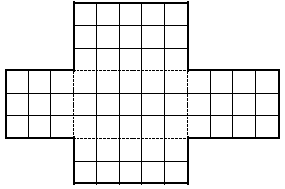
\includegraphics[scale=0.35]{13.png}}
\end{figure}
\end{center}
70. Один литр --- это кубический дециметр. На уроке труда Вася сделал стальную заготовку для ванны с прямоугольным основанием, изображённую на схеме (пунктирные линии обозначают места сгиба). Сторона одной клеточки равна 1 дециметру. Сварив края ванны, Вася обнаружил, что она вышла кривая. Какое наибольшее количество литров воды войдёт в ванну?
\begin{center}
\begin{figure}[ht!]
\center{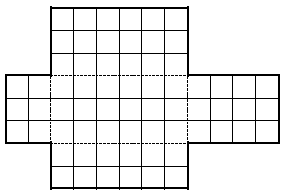
\includegraphics[scale=0.35]{133.png}}
\end{figure}
\end{center}

ewpage

oindent
71. На рисунке изображена буква О ширины 5, высоты 7, толщины 2 клетки. Суммарная длина её внутренних перегородок равна 48. Чему равна суммарная длина внутренних перегородок буквы О, у которой толщина 4, высота 40, ширина 30 клеток?
\begin{center}
\begin{figure}[ht!]
\center{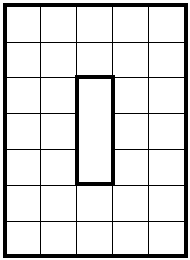
\includegraphics[scale=0.35]{14.png}}
\end{figure}
\end{center}
72. На рисунке изображена буква О ширины 5, высоты 7, толщины 2 клетки. Суммарная длина её внутренних перегородок равна 48. Чему равна суммарная длина внутренних перегородок буквы О, у которой толщина 4, высота 30, ширина 20 клеток?
\begin{center}
\begin{figure}[ht!]
\center{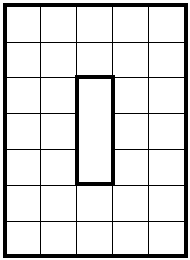
\includegraphics[scale=0.35]{14.png}}
\end{figure}
\end{center}
73. В большую квадратную комнату внесли два квадратных ковра. Сторона одного из ковров в два раза больше стороны другого. Оказалось, что если положить ковры в противоположные углы комнаты, то они покроют в два слоя участок пола площадью $4\text{м}^2.$ А если положить ковры в соседние углы комнаты, то в два слоя окажется покрыт участок площадью $14\text{м}^2.$ Чему равна сторона комнаты?\\
74. В большую квадратную комнату внесли два квадратных ковра. Сторона одного из ковров в два раза больше стороны другого. Оказалось, что если положить ковры в противоположные углы комнаты, то они покроют в два слоя участок пола площадью $9\text{м}^2.$ А если положить ковры в соседние углы комнаты, то в два слоя окажется покрыт участок площадью $15\text{м}^2.$ Чему равна сторона комнаты?\\
75. Сумма двух чисел равна 8481. Одно из них оканчивается нулём. Если этот нуль зачеркнуть, то получится второе число. Найдите эти числа.\\
76. Будем говорить, что прямоугольника имеет пузатость $2:1,$ если одна его сторона в два раза больше другой. А у прямоугольника со сторонами 3см и 2см пузатость равна $3:2.$ Было два прямоугольника, у каждого из которых пузатость равнялась $4:1.$ Из них сложили один прямоугольник. Чему может быть равна его пузатость?\\
77. Будем говорить, что прямоугольника имеет пузатость $2:1,$ если одна его сторона в два раза больше другой. А у прямоугольника со сторонами 3см и 2см пузатость равна $3:2.$ Было два прямоугольника, у каждого из которых пузатость равнялась $3:1.$ Из них сложили один прямоугольник. Чему может быть равна его пузатость?\\
78. Сколько существует таких натуральных чисел $N,$ для которых {\bf ровно одно} из чисел $N$ и $N+937$ трёхзначное?\\
79. Сколько существует таких натуральных чисел $N,$ для которых {\bf ровно одно} из чисел $N$ и $N+973$ трёхзначное?\\
80. Сколько существует чётных пятизначных чисел с произведением цифр 20?\\
81. Сколько существует чётных пятизначных чисел с произведением цифр 28?\\
82. На электронных часах высвечивается 13:00:07. Через какое время впервые все цифры на табло часов окажутся разными?\\
83. На электронных часах высвечивается 12:00:08. Через какое время впервые все цифры на табло часов окажутся разными?\\
84. В трёх пассажирских поездах различное число мест: 236, 295, 472. Во всех вагонах число мест одинаковое и большее 30. Сколько вагонов в этих поездах вместе?\\
85. В трёх пассажирских поездах различное число мест: 265, 318, 477. Во всех вагонах число мест одинаковое и большее 30. Сколько вагонов в этих поездах вместе?\\
86. На рисунке изображены две клетчатые фигуры: прямоугольник $7\times8$ с дыркой и буква $L$ странной формы. У каждой из фигур одна клетка отмечена чёрным. Эти фигуры по клеточкам положили на тетрадный лист так, что чёрные клетки находятся в точности друг над другом. Клетки фигуры и клетки листа совпадают. Фигурки можно поворачивать и переворачивать. Алина посчитала, сколько клеток тетрадного листа накрыто хотя бы одной из фигурок. Какие числа она могла получить? В ответ запишите {\bf все возможные} варианты через запятую.
\begin{center}
\begin{figure}[ht!]
\center{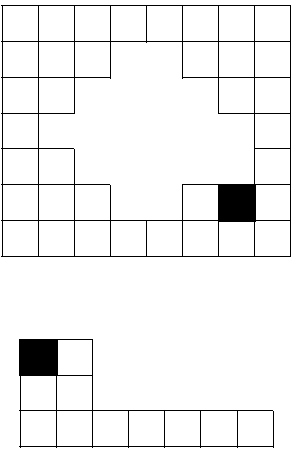
\includegraphics[scale=0.35]{15.png}}
\end{figure}
\end{center}
87. На рисунке изображены две клетчатые фигуры: прямоугольник $7\times9$ с дыркой и буква $P$ странной формы. У каждой из фигур одна клетка отмечена чёрным. Эти фигуры по клеточкам положили на тетрадный лист так, что чёрные клетки находятся в точности друг над другом. Клетки фигуры и клетки листа совпадают. Фигурки можно поворачивать и переворачивать. Алина посчитала, сколько клеток тетрадного листа накрыто хотя бы одной из фигурок. Какие числа она могла получить? В ответ запишите {\bf все возможные} варианты через запятую.
\begin{center}
\begin{figure}[ht!]
\center{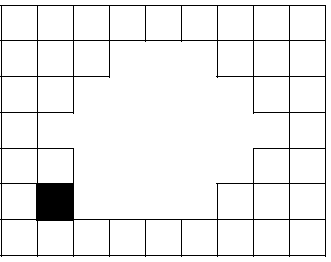
\includegraphics[scale=0.35]{155.png}}
\center{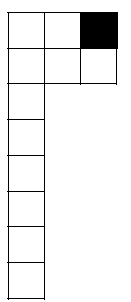
\includegraphics[scale=0.35]{156.png}}
\end{figure}
\end{center}
88. Миша выбирает какие-нибудь три года из XXI века, перемножает цифры каждого года и складывает полученные произведения. Какое самое большое число он может получить?\\
89. Зоя выбирает какие-нибудь три года из XXI века, перемножает цифры каждого года и складывает полученные произведения. Какое самое большое число она может получить?\\
90. Некоторые из городов A, B, C, D и E соединены между собой дорогами. Любые два города соединены не более, чем одной дорогой (может и не быть дороги, ведущей напрямую из одного города в другой). Из города A выходят 4 дороги, из городов B и E по 2 дороги, из городов C и D по 3 дороги. Из следующих утверждений выберите ровно одно верное:\\
А) Из города A нельзя напрямую попасть в город D;\\
Б) Из города B нельзя напрямую попасть в город E;\\
В) Из города D можно напрямую попасть и в город B, и в город E.\\
Г) Из города C можно напрямую попасть либо в город А, либо в город D.\\
91. Некоторые из городов К, Л, М, Н и О соединены между собой дорогами. Любые два города соединены не более, чем одной дорогой (может и не быть дороги, ведущей напрямую из одного города в другой). Из города О выходят 4 дороги, из городов К и Л по 2 дороги, из городов М и Н по 3 дороги. Из следующих утверждений выберите ровно одно верное:\\
А) Из города О нельзя напрямую попасть в город Л;\\
Б) Из города Л нельзя напрямую попасть в город К;\\
В) Из города Н можно напрямую попасть и в город К, и в город Л.\\
Г) Из города М можно напрямую попасть либо в город Н, либо в город О.\\
92. Шерлок Холмс получил записку, в которой сказано: {\it <<Барон М. солгал, когда сказал, что неправда, что А и Б одновременно сидели на трубе.>>} В этой записке написана ложь. Это означает, что:\\
А) А и Б одновременно сидели на трубе;\\
Б) На трубе обязательно сидел только Б;\\
В) А и Б не сидели на трубе одновременно;\\
Г) Б совершенно точно не сидел на трубе.\\
93. Доктор Ватсон получил записку, в которой сказано: {\it <<Кучер обманул Вас, когда сказал, что неправда, что А и Б одновременно НЕ сидели на трубе.>>} В этой записке написана ложь. Это означает, что:\\
А) А и Б одновременно сидели на трубе;\\
Б) На трубе обязательно сидел только Б;\\
В) А и Б не сидели на трубе одновременно;\\
Г) Б совершенно точно не сидел на трубе.\\
94. Крокодил Гена разложил по четырём коробкам нужные вещи. В одной коробке у него лежали лампочки, в другой гвозди, в третьей нитки и иголки, в четвёртой нитки и лампочки. Для коробок он приготовил этикетки: Л, Г, НИ, НЛ. Пока он отвернулся, Шапокляк приклеила этикетки так, что ничего из упомянутого на этикетке не находится в коробке, на которую она наклеена. Что лежит в коробке с этикеткой Л?\\
95. Знайка разложил по четырём коробкам нужные вещи. В одной коробке у него лежали шапочки, в другой тапочки, в третьей книжки и блокноты, в четвёртой книжки и шапочки. Для коробок он приготовил этикетки: Ш, Т, КБ, КШ. Пока он отвернулся, Незнайка приклеил этикетки так, что ничего из упомянутого на этикетке не находится в коробке, на которую она наклеена. Что лежит в коробке с этикеткой Т?\\
96. Найдите наименьшее трёхзначное число, которое делится на 3, и первая цифра которого равна 4.\\
97. В коробке лежат 100 синих и 100 красных шаров. Какое наименьшее число шаров надо вытащить, не заглядывая в коробку, чтобы среди них наверняка было 5 шаров одного цвета?\\
98. Какие четыре цифры надо вычеркнуть из числа 5837609, чтобы получившееся трёхзначное число было как можно меньше?\\
99. Из чисел 2, 3, 8, 18, 92, 238, 568 выберите делимое, делитель, частное и остаток.\\
100. Используя только цифры 0, 2, 3, 4 запишите такое наименьшее шестизначное число, чтобы каждая из цифр 0, 2, 3, 4 в нём присутствовала.\\
101. На рисунке изображена развёртка игрального кубика. Сумма цифр на любых двух противоположных гранях равна 7. Какой может быть наибольшая разность цифр на закрашенных гранях? Напоминаем, что на всех гранях стоят разные цифры от 1 до 6.
\begin{center}
\begin{figure}[ht!]
\center{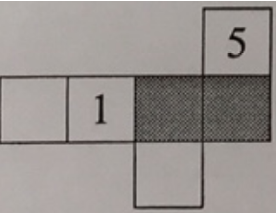
\includegraphics[scale=0.35]{17.png}}
\end{figure}
\end{center}
102. У Саши 20 кубиков, у Васи 27 кубиков, у Вани 18 кубиков, а у Олега --- 10 кубиков. Кто из мальчиков может построить куб из всех своих кубиков?\\
103. На пикник отправились пятеро мужчин из одной семьи: дедушка, два его сына и два внука. Их зовут: Олег Игоревич, Николай Олегович, Игорь Николаевич, Василий Александрович и Александр Игоревич. Какое имя у дедушки?
ewpage

oindent104. На рисунке изображена развёртка игрального кубика. Сумма цифр на любых двух противоположных гранях равна 7. Какой может быть наибольшая разность цифр на закрашенных гранях? Напоминаем, что на всех гранях стоят разные цифры от 1 до 6.
\begin{center}
\begin{figure}[ht!]
\center{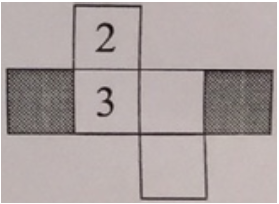
\includegraphics[scale=0.35]{177.png}}
\end{figure}
\end{center}
105. На рисунке изображены несколько верёвок. На каких из них завяжется узел, если потянуть их за концы?
\begin{center}
\begin{figure}[ht!]
\center{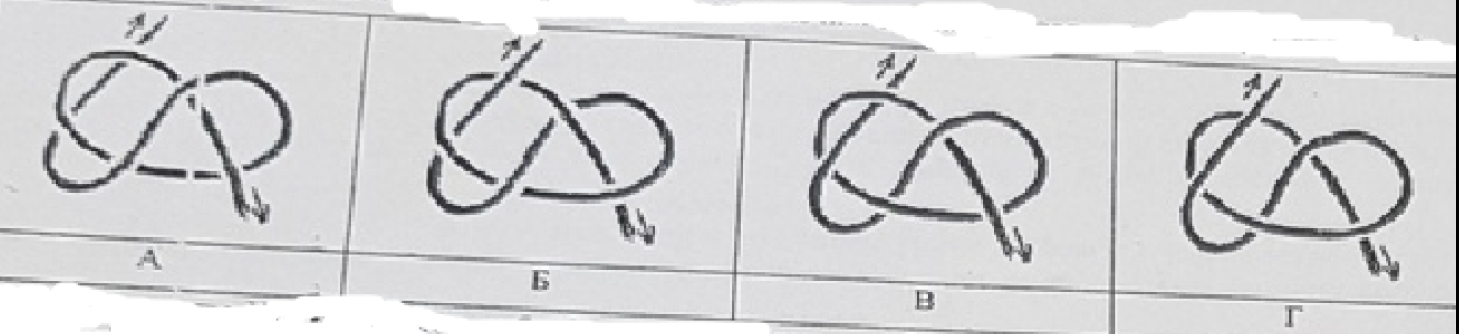
\includegraphics[scale=0.35]{18.png}}
\end{figure}
\end{center}
106. На рисунке изображены несколько верёвок. На каких из них завяжется узел, если потянуть их за концы?
\begin{center}
\begin{figure}[ht!]
\center{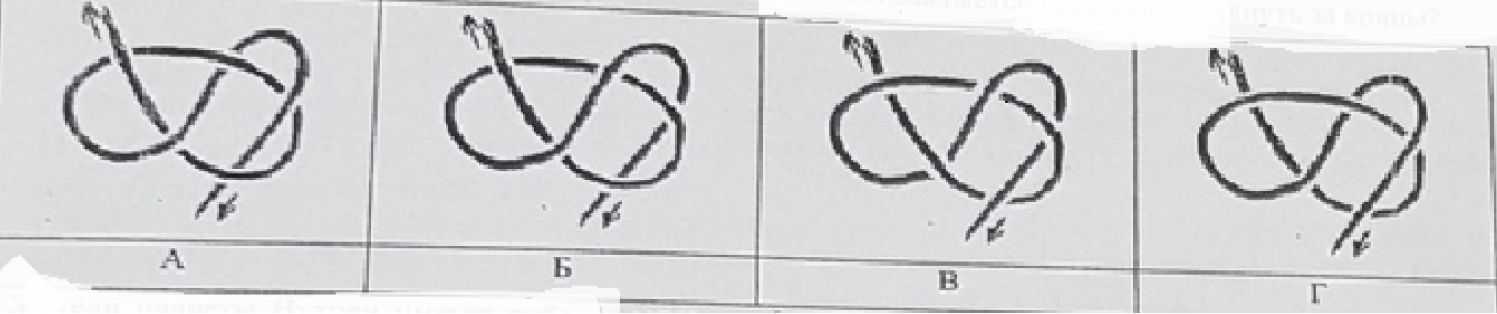
\includegraphics[scale=0.35]{188.png}}
\end{figure}
\end{center}
107. Соловей-разбойник, попав в темницу, рассказывал, что в схватке ему удалось победить Алёшу Поповича, или Добрыню Никитича, или даже обоих. При этом Соловей-разбойник как обычно врал. Как же обстояли дела на самом деле? Выберите {\it все} возможные варианты произошедшего.\\
А) Возможно, Соловья-разбойника пленил Илья Муромец;\\
Б) Возможно, Соловей-разбойник победил Алёшу, но не Добрыню;\\
В) Возможно, Соловей-разбойник победил Добрыню, но не Алёшу;\\
Г) Ни Добрыня, ни алёша не были побеждены Соловьём-разбойником.\\
108. Баба Яга рассказывала, что на конкурсе красоты она победила Василису Прекрасную, или Василису Премудрую, или даже обеих. При этом Баба Яга как обычно врала. Как же обстояли дела на самом деле? Выберите {\it все} возможные варианты произошедшего.\\
А) Возможно, Баба Яга победила Василису Прекрасную, но не Василису Премудрую;\\
Б) Возможно, Баба Яга победила Василису Премудрую, но не Василису Прекрасную;\\
В) Ни одна Василиса не была побеждена Бабой Ягой;\\
Г) Возможно, Баба Яга победила Кикимору Болотную.\\
109. Оля отправила по почте 2 письма Зое. Изначально у Оли было 6 марок, которые стоили 18 рублей, 21 рубль, 24 рубля, 27 рублей, 30 рублей и 33 рубля. После отправки у Оли осталась одна марка. Какая марка осталась, если письма стоили одинаково?\\
110. Алёша отправил по почте 2 письма Олегу. Изначально у Алёши было 6 марок, которые стоили 20 рублей, 24 рубля, 28 рублей, 32 рубля, 36 рублей и 40 рублей. После отправки у Алёши осталась одна марка. Какая марка могла остаться, если письма стоили одинаково?

ewpage

oindent111. Из одинаковых кубиков склеена фигура. Её сфотографировали спереди, сверху и справа. Каким может быть максимальное количество кубиков в этой фигуре?
\begin{center}
\begin{figure}[ht!]
\center{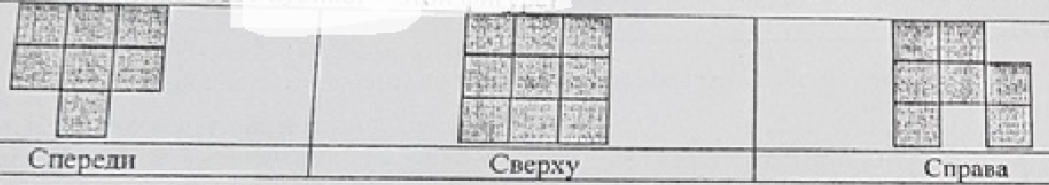
\includegraphics[scale=0.35]{19.png}}
\end{figure}
\end{center}
112. Из одинаковых кубиков склеена фигура. Её сфотографировали спереди, сверху и слева. Каким может быть максимальное количество кубиков в этой фигуре?
\begin{center}
\begin{figure}[ht!]
\center{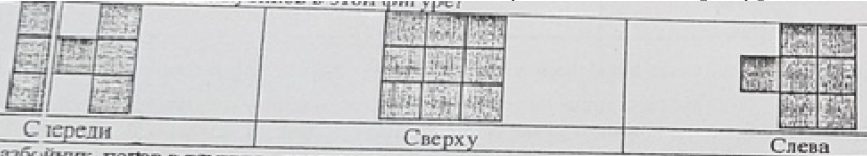
\includegraphics[scale=0.35]{199.png}}
\end{figure}
\end{center}
113. Запишите четырёхзначное число, в котором число десятков вдвое меньше, чем число тысяч; если число сотен умножить на число тысяч, то число сотен не изменится; число единиц на 7 больше числа тысяч.\\
114. Запишите четырёхзначное число, в котором число сотен втрое меньше, чем число тысяч; если число десятков умножить на число тысяч, то число десятков не изменится; число единиц на 5 больше числа тысяч.\\
115. Нарисуйте недостающие фигурки в пустых клетках.
\begin{center}
\begin{figure}[ht!]
\center{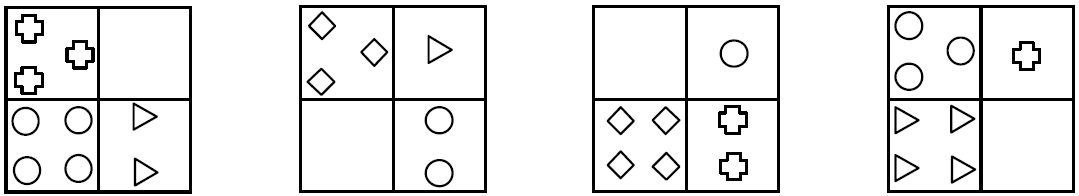
\includegraphics[scale=0.35]{20.png}}
\end{figure}
\end{center}
116. Фукс пообещал капитану Врунгелю, что выучит испанский язык или побывает на полюсе. Пока Фукс не выполнил своё обещание. Это означает, что он\\
а) выучил испанский язык, но пока не был на полюсе;\\
б) не выучил испанский язык и на полюсе пока не был;\\
в) побывал а полюсе, но испанский пока не выучил;\\
г) выучил испанский и побывал на полюсе.\\
117. На рисунке изображена развёртка куба. Рядом изображён куб, собранный из этой же развёртки. Сколько точек на той грани, которой этот куб стоит на столе?
\begin{center}
\begin{figure}[ht!]
\center{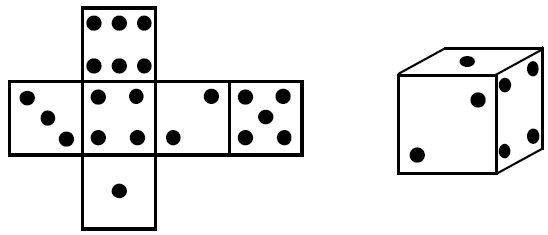
\includegraphics[scale=0.35]{21.png}}
\end{figure}
\end{center}
118. Муравьишка ползает по клетчатому полю $5\times5$ клеток. Он начинает свой путь в правой верхней клетке. Оттуда он ползёт на 2 клетки влево, потом на 4 клетки вниз, потом на 1 клетку вправо, потом на 2 клетки вверх, потом на 3 клетки влево, потом на 1 клетку вверх, потом на 4 клетки вправо, потом на 2 клетки вниз, потом на 3 клетки влево, потом на 2 клетки вверх, потом на 1 клетку вправо, потом на 1 клетку вверх, и оттуда на 2 клетки вправо. Муравьишка не перепрыгивает через клетки на своём пути. В скольких клетках Муравьишка не побывал за время своего путешествия?\\
119. Электронное табло сделано из ламп, как показано на рисунке. На табло меняются числа от 00 до 99. Например, на рисунке показано число 72. Сколько раз в одной из цифр будет гореть на 2 лампы больше, чем в другой?
\begin{center}
\begin{figure}[ht!]
\center{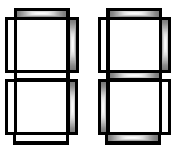
\includegraphics[scale=0.35]{222.png}}
\end{figure}
\end{center}
120. Вася построил большой куб из кубиков. Потом он убрал часть кубиков из всех слоёв, кроме нижнего. Теперь каждый слой кубиков имеет форму квадрата, а сбоку конструкция выглядит так, как на рисунке. сколько кубиков убрал Вася?
\begin{center}
\begin{figure}[ht!]
\center{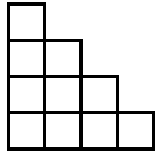
\includegraphics[scale=0.35]{333.png}}
\end{figure}
\end{center}
121. Нарисуйте на клетчатой бумаге какой-нибудь десятиугольник с площадью десять с половиной $\text{см}^2.$ Сторона клетки --- половина сантиметра.\\
122. Садовник Порфирий решил посадить вишнёвый сад на участке длиной 200 м, шириной 100 м. Для этого весь участок он разделил на квадраты $10\times10$ м. В центр каждого такого квадрата и в место, где соединяются границы четырёх квадратов, он посадил саженец вишни. Сколько саженцев понадобилось Порфирию?\\
123. В магазине продавали футболки, кепки и шорты: красные и синие. К концу рабочего дня много товара продали, и оказалось, что все оставшиеся кепки синие, а из красных вещей остались только футболки. Какие из утверждений наверняка верны (их может быть несколько или не быть совсем)? К концу рабочего дня: 1) Нет красных кепок. 2) Все футболки красные. 3) Все кроссовки зелёные. 4) Все шорты синие. 5) Некоторые футболки синие.\\
124. Сколько существует четырёхзначных чисел, у которых сумма цифр равна 3?\\
125. Сколько существует четырёхзначных чисел, у которых сумма цифр равна 34?\\
126. У треугольника отмечены вершины и середины двух сторон. Сколько существует треугольников, вершины которых лежат в отмеченных точках?\\
127. На отрезке AD длиной 33 сантиметра стоят точки B и C так, что: точки расположены в порядке ABCD; отрезок BC в два раза длиннее отрезка AB, а отрезок CD --- в 4 раза длиннее BC. Найдите длины отрезков AB, BC и CD.\\
128. На отрезке AD длиной 25 сантиметров стоят точки B и C так, что: точки расположены в порядке ACBD; отрезок BC в два раза короче отрезка AB, а отрезок CD --- в 4 раза длиннее BC. Найдите длины отрезков AC, CB и BD.\\
129. На острове рыцарей и лжецов живут два брата-близнеца --- Марк и Лев. Один из них лжец, а другой рыцарь. Лжецы всегда лгут, а рыцари всегда говорят правду. В день рождения братьев Марк сказал гостям: <<Теперь мне больше десяти лет!>> Лев в тот же день заявил, что ему больше девяти лет. Сколько лет близнецам?\\
130. На острове рыцарей и лжецов живут два брата-близнеца --- Рон и Тук. Один из них лжец, а другой рыцарь. Лжецы всегда лгут, а рыцари всегда говорят правду. В день рождения братьев Рон сказал гостям: <<Теперь мне больше двенадцати лет!>> Тук в тот же день заявил, что ему больше одиннадцати лет. Сколько лет близнецам?\\
131. Со стола на кухне пропала конфета. Мама спросила у троих своих детей: <<Кто взял конфету?>> Аня сказала, что конфету взял Борис. Борис и Вика тоже что-то ответили, но мама не запомнила их ответы. Всё же мама выяснила, что конфету взял один из детей и что только он сказал правду. Кто взял конфету?\\
132. Мама купила коробку сахара-рафинада. Пока её не было дома, дети сначала съели верхний слой --- 77 кусочков, затем боковой слой --- 55 кусочков. И, наконец, съели передний слой. Сколько кусочков сахара дети съели в третий раз?\\
133. Бабушка принесла из магазина коробку сахара-рафинада. Пока её не было дома, дети сначала съели верхний слой --- 55 кусочков, затем боковой слой --- 33 кусочка. Сколько кусочков сахара осталось?\\
134. Произведение цифр четырёхзначного числа равно 210, сумма первой и второй цифр --- 8, произведение второй и третьей --- 21. Найдите эти числа.\\
135. Робот LR90 проделал следующие действия:\\
1) прошёл прямо 2 метра и повернул налево на $90^\circ$;\\
2) прошёл прямо 1 метр, провернул направо на $90^\circ,$ прошёл прямо ещё 1 метр и повернул налево на $90^\circ$;\\
3) повторил действие (2) ещё 4 раза;\\
4) прошёл прямо 1 метр и повернул налево на $90^\circ$;\\
5) повторил действие (1) 1 раз;\\
6) повторил действие (2) 5 раз;\\
7) прошёл прямо 1 метр.\\
Нарисуйте путь робота и найдите площадь фигуры, которую он ограничивает.\\
136. Робот LR90 проделал следующие действия:\\
1) прошёл прямо 2 метра и повернул налево на $90^\circ$;\\
2) прошёл прямо 2 метра, провернул направо на $90^\circ,$ прошёл прямо ещё 1 метр и повернул налево на $90^\circ$;\\
3) повторил действие (2) ещё 2 раза;\\
4) прошёл прямо 1 метр и повернул налево на $90^\circ$;\\
5) повторил действие (1) 1 раз;\\
6) повторил действие (2) 3 раза;\\
7) прошёл прямо 1 метр.\\
Нарисуйте путь робота и найдите площадь фигуры, которую он ограничивает.\\
137. Нарисуйте, как из данных трёх фигурок, использовав каждую ровно один раз, сложить фигуру, имеющую ось симметрии.
\begin{center}
\begin{figure}[ht!]
\center{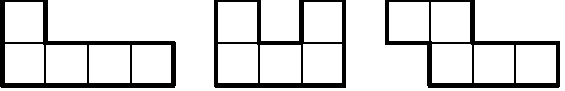
\includegraphics[scale=0.35]{34.png}}
\end{figure}
\end{center}
138. Представьте число 533533533533 в виде произведения как можно большего числа различных натуральных сомножителей.\\
139. Представьте число 517517517517 в виде произведения как можно большего числа различных натуральных сомножителей.\\
140. Четыре спортсмена участвовали в забеге. Оказалось, что Иванов прибежал раньше Петрова, а Васильев --- позже Борисова. Обведите заведомо ложные утверждения:\\
а) Забег выиграл Васильев;\\
б) Иванов прибежал раньше Борисова;\\
в) Последним прибежал не Иванов и не Васильев;\\
г) Если Петров прибежал раньше Васильева, то Петров был последним.\\
141. Четыре толстяка соревновались, кто больше съест пирожных. Оказалось, что Дмитрий съел больше, чем Алексей, а Сергей --- меньше, чем Борис. Обведите заведомо истинные утверждения:\\
а) Алексей съел меньше всех пирожных;\\
б) Дмитрий съел больше, чем Борис;\\
в) Меньше всех съел не Дмитрий и не Сергей;\\
г) Если Алексей съел больше Бориса, то Сергей съел меньше всех.\\
142. У квадрата со стороной 20 см вырезали внутреннюю часть, оставив только каёмку шириной две клеточки. Сколько клеток в этой каёмке? Сторона одной клеточки равна половине сантиметра.\\
143. У квадрата со стороной 17 см вырезали внутреннюю часть, оставив только каёмку шириной три клеточки. Сколько клеток в этой каёмке? Сторона одной клеточки равна половине сантиметра.\\
144. Нарисуйте по сторонам клеточек фигурку, которую можно одним прямолинейным разрезом разделить на пять одинаковых частей. Покажите, как должен идти разрез.\\
145. Нарисуйте по сторонам клеточек фигурку, которую можно одним прямолинейным разрезом разделить на четыре одинаковых части. Покажите, как должен идти разрез.\\
146. В числе 3728924106 зачеркнуть три цифры так, чтобы оставшиеся цифры в том же порядке составили бы наименьшее число. После зачёркивания записать число, которое получается в результате.\\
147. Сколько существует таких пар натуральных чисел $N$ и $N+6,$ что ровно одно из них трёхзначное?\\
148. Вставьте вместо звёздочки цифру так, чтобы 3*44 делилось на 18.\\
149. Начертите прямую и расставьте на ней точки A, B, C и D так, чтобы AB=8 см, CB=5 см, DC=1 см, AC=3 см.\\
150. Сколько треугольников изображено на чертеже?
\begin{center}
\begin{figure}[ht!]
\center{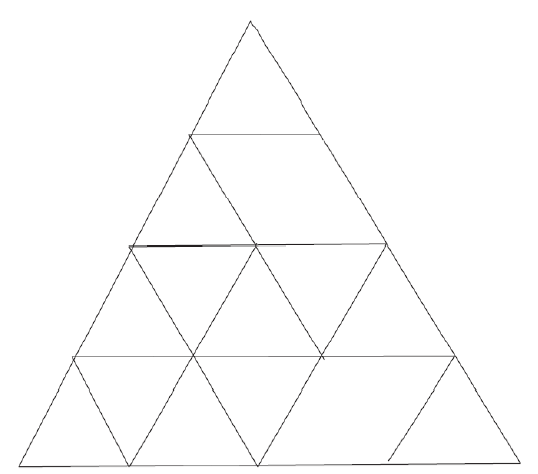
\includegraphics[scale=0.35]{35.png}}
\end{figure}
\end{center}
151. Перечислите все треугольники, которые есть на рисунке.
\begin{center}
\begin{figure}[ht!]
\center{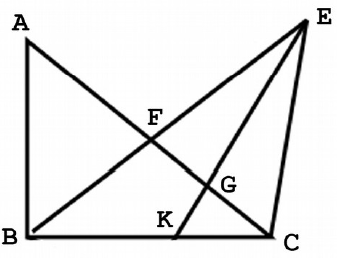
\includegraphics[scale=0.35]{36.png}}
\end{figure}
\end{center}
152. Назовём натуральное число <<замечательным>>, если оно самое маленькое среди натуральных чисел с такой же, как у него, суммой цифр. Чему равно 2017-е <<замечательное>> число?\\
153. Мама купила коробку сахара. дети сначала съели передний слой в 44 кусочка, затем верхний слой --- 77 кусочков и, наконец, боковой слой. Сколько кусочков сахара съели дети? Сколько кусочков сахара было в коробке?\\
154. Екатерина Михайловна покупает тетради для олимпиады. В олимпиаде будет участвовать не то 176 детей, не то 256 детей, она точно не помнит. В магазине есть пачки с любым количеством тетрадей от 2 до 50. Какие пачки следует выбрать Екатерине Михайловне, чтобы купить как можно меньше пачек и на олимпиаде было израсходовано целое число пачек?\\
155. Прямоугольный лист бумаги разделили на четыре части, одна из которых --- квадрат. Периметры серых прямоугольников равны 34 см и 22 см. Найдите: а) периметр; б) площадь листа бумаги.
\begin{center}
\begin{figure}[ht!]
\center{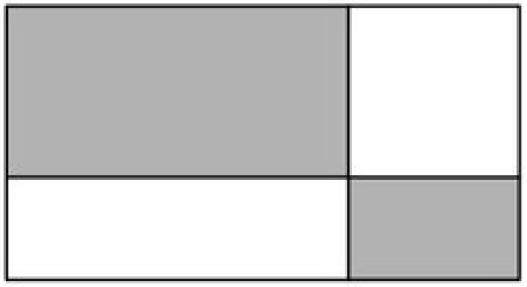
\includegraphics[scale=0.35]{37.png}}
\end{figure}
\end{center}
ewpage
oindent
156. Мальвина велела Буратино вместо звёздочек написать различные цифры от 1 до 9 так, чтобы сумма цифр в каждом круге равнялась бы 13. Одну цифру Буратино написал. Помогите ему расставить остальные.
\begin{center}
\begin{figure}[ht!]
\center{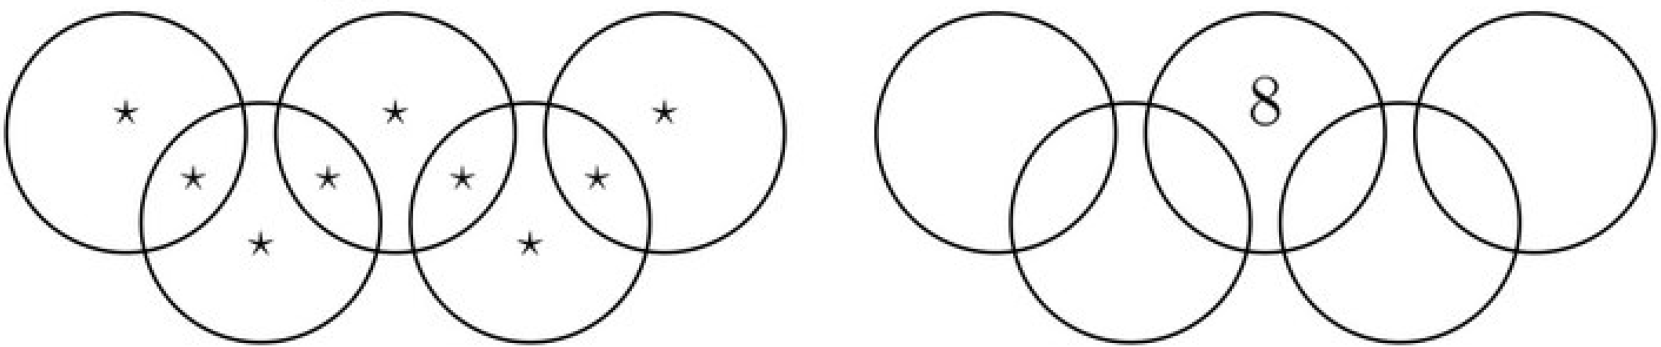
\includegraphics[scale=0.35]{38.png}}
\end{figure}
\end{center}
157. В ящике лежат 100 синих, 100 красных, 100 зелёных и 100 фиолетовых карандашей. Сколько карандашей необходимо достать, не заглядывая в ящик, чтобы среди них обязательно нашлись по крайней мере 1 красный и 1 фиолетовый?\\
158. В стране Лимпопо 9 городов и каждые два города соединены авиалинией. Сколько всего авиалиний в стране Лимпопо?\\
159. Сколько имеется пятизначных чисел, сумма цифр в которых равна трём, причём цифра 1 в записи каждого числа встречается не более одного раза?\\
160. В доме, который заселён только супружескими парами с детьми, проводилась перепись населения. Недобросовестный человек, проводивший перепись, в отчёте указал: <<Взрослых в доме больше, чем детей. У каждого мальчика есть сестра. Мальчиков больше, чем девочек. Бездетных семей нет.>> Найдите в этом отчёте
как можно больше нестыковок и объясните их.\\
161. Расшифруйте ребус на картинке и объясните своё решение.
\begin{center}
\begin{figure}[ht!]
\center{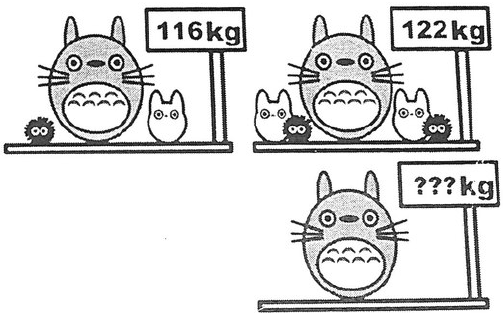
\includegraphics[scale=0.35]{39.png}}
\end{figure}
\end{center}
162. На гранях кубика написаны буквы А, Б, В, Г, Д, Е. На каждой грани 1 буква, при этом все буквы встречаются по 1 разу. Если посмотреть на кубик с одной стороны, то можно увидеть буквы А, В, Г, а если посмотреть ещё с одной стороны, можно увидеть грани Д, Б, В. Какая буква находится на грани, противоположной грани с буквой Е?\\
163. Разделите фигуру на рисунке на 2 одинаковые части.
\begin{center}
\begin{figure}[ht!]
\center{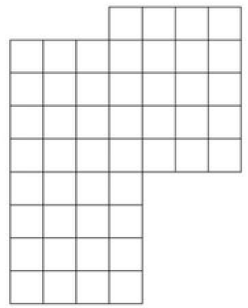
\includegraphics[scale=0.35]{40.png}}
\end{figure}
\end{center}
164. В коробке 30 шариков и кубиков. Среди любых 12 предметов имеется хотя бы один шарик, а среди любых 20 предметов имеется хотя бы один кубик. Сколько шариков и сколько кубиков в коробке?\\
165. Расставьте 8 минусов и 17 плюсов в клетках квадрата $5\times5$ так, чтобы рядом с каждым минусом (т.е. в клетках, соседних по стороне) было ровно 2 плюса.\\
166. Существуют ли два последовательных натуральных числа, сумма цифр каждого из которых делится на 7?\\
167. Пятнадцать рабочих собрали 100 компьютеров. Верно ли, что какие-то два из них собрали одинаковое число компьютеров?\\
168. Выпишите все двузначные числа, которые можно записать с помощью цифр 1, 0 и 3, используя каждую цифру по одному разу. Найдите сумму этих чисел.\\
169. На отрезке AB, равном 32 см, выбрана точка L так, что AL=28 см, и точка K так, что BK=22 см. Найдите отрезок LK.\\
170. В числе 92574063 зачеркните три цифры так, чтобы оставшиеся пять цифр в той же последовательности образовывали как можно меньшее число.\\
171. Есть 6 карточек с цифрой 2. Используя все эти карточки, знаки арифметических действий и, если нужно, скобки, получите число 55.\\
172. Расставь скобки так, чтобы равенство стало верным:\\
а) $7200:90-10\cdot6=540.$\\
б) $8400:3\cdot40+20=90.$\\
в) $210-30:5\cdot3=12.$\\
173. Сколько чётных чисел можно составить, если использовать только цифры 0, 1, 3, 5, причём каждую не более одного раза?\\
174. Сколько различных трёхзначных чисел можно составить из цифр 1, 2, 3, 4?\\
175. Наступил 2017 год. Сколько годов с такой же суммой цифр будет в ближайшие 100 лет?\\
176. В стране Лимпопо 5 городов. Каждые 2 города соединены авиалинией. Сколько всего авиалиний в стране Лимпопо?\\
177. В лавке старьевщика Аладдин увидел три древние лампы: золотую, серебряную и бронзовую, в которых жили добрый и злой джинны. Надпись на золотой лампе гласила: «Здесь живет добрый джинн». На серебряной была надпись «Бронзовая лампа пустая». На бронзовой лампе было написано «Здесь живёт злой джинн». Какую лампу должен выбрать Аладдин, если ему нужен добрый джинн, а все надписи неправильные?\\
178. В одном доме живут четыре друга. Владимир и шофёр старше Сергея. Никита и слесарь занимаются боксом. Электрик – младший из друзей. По вечерам Андрей и токарь играют в лото против Сергея и электрика. Определите профессию каждого из друзей.\\
179. В осеннем лесу росли грибы: мухоморы и белые. Стадо ёжиков прокатилось по грибной полянке и унесло на своих иголках богатую грибную добычу. Внимательная ворона заметила: ёжики унесли столько белых грибов, сколько мухоморов осталось на полянке. Чего было больше: мухоморов, которые сначала росли на полянке, или всех грибов, которые унесли ёжики?\\
180. Вася посчитал число коробочек, в которых один шарик или больше: их оказалось 8; коробочек, в которых больше одного шарика --- 6; больше двух шариков --- 5; больше трёх --- 3; больше четырёх --- 2. Коробочек, в которых больше пяти шариков, не было. Найдите общее число шариков во всех коробках.\\
181. Седьмая часть всех попугаев умеет говорить; пятая часть всех говорящих животных --- попугаи. Кого больше: попугаев или говорящих животных?\\
182. Шестнадцать мальчишек собрались на рыбалку. Известно, что каждый мальчишка, который надел сапоги, надел и кепку. Без сапог оказалось 10 мальчишек, а без кепки --- двое. Каких мальчишек и на сколько больше: тех, кто был в кепке, но без сапог, или тех, кто надел сапоги?\\
183. На лужайке босоногих мальчиков столько же, сколько обутых девочек. Кого на лужайке больше, девочек или босоногих детей?\\
184. В день рождения дяди Фёдора почтальон Печкин хочет выяснить, сколько тому лет. Шарик говорит, что дяде Фёдору больше 11 лет, а кот Матроскин утверждает, что больше 10 лет. Сколько лет дяде Фёдору, если известно, что ровно один из них ошибся?\\
185. Однажды на лестнице была найдена странная тетрадь. В ней было записано сто утверждений:\\
<<В этой тетради ровно одно неверное утверждение>>;\\
<<В этой тетради ровно два неверных утверждения>>;\\
<<В этой тетради ровно три неверных утверждения>>;\\
...\\
<<В этой тетради ровно сто неверных утверждений>>.\\
Есть ли среди этих утверждений верные, и если да, то какие?\\
186. Мачеха, уезжая на бал, дала Золушке мешок, в котором были перемешаны мак и просо, и велела перебрать их. Когда Золушка уезжала на бал, она оставила три мешка: в одном было просо, в другом --- мак, а в третьем --- ещё не разобранная смесь. Чтобы не перепутать мешки, Золушка к каждому из них прикрепила по табличке: <<Мак>>, <<Просо>> и <<Смесь>>. Мачеха вернулась с бала первой и нарочно поменяла местами все таблички так, чтобы на каждом мешке оказалась неправильная надпись. Ученик Феи успел предупредить Золушку, что теперь ни одна надпись на мешках не соответствует действительности. Тогда Золушка достала только одно-единственное зёрнышко из одного мешка и, посмотрев на него, сразу догадалась, где что лежит. Как она это сделала?\\
187. Среди математиков каждый седьмой --- философ, а среди философов каждый девятый --- математик. Кого больше: философов или математиков?\\
188. Прямоугольник периметра 536 см разрезали на два прямоугольника. У одного из новых прямоугольников периметр равен 320 см, а у другого --- 410 см. Найдите площадь того из новых прямоугольников, у кого она меньше.\\
189. Прямоугольник ABCD разделили двумя прямолинейными разрезами на четыре прямоугольника. Известно, что периметр прямоугольника AKFE равен 29 см, периметр прямоугольника EFGD равен 15 см,  а периметр прямоугольника KBHF равен 36 см. Найдите периметр прямоугольника FHCG.\\
190.  К прямоугольнику с двух противоположных сторон приклеили равные квадраты так, что получился новый прямоугольник. Периметр получившегося прямоугольника оказался на 52 см больше периметра первоначального прямоугольника. Найдите периметр каждого квадрата и объясните своё решение.\\
191. Прямоугольник ABCD разделили на четыре меньших прямоугольника с одинаковыми периметрами. Известно, что AB = 18 см, а BC = 16 см. Найдите длины сторон остальных прямоугольников. Обязательно объясните свой ответ.
\begin{center}
\begin{figure}[ht!]
\center{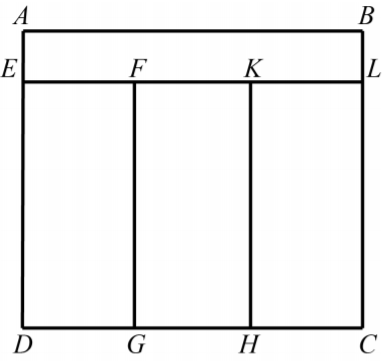
\includegraphics[scale=0.35]{41.png}}
\end{figure}
\end{center}
192. Расстояние между деревнями Орехово и Горохово равно 3 км. В деревне Орехово живут 300 школьников, в деревне Горохово --- 200 школьников. Где следует построить школу, чтобы общее расстояние, пройденное всеми школьниками по дороге в школу, было как можно меньше?\\
193. В деревне A живет 100 школьников, в деревне B живет 50 школьников. Расстояние между деревнями 3 километра. 
В какой точке дороги из A в B надо построить школу, чтобы суммарное расстояние, проходимое всеми школьниками, было бы как можно меньше?\\
194. В ящике красные и жёлтые яблоки. Сколько попыток нужно, чтобы вытащить 2 яблока одного цвета?\\
195. В ящике по 12 яблок красного, жёлтого и зелёного цвета. Сколько попыток дадут 3 яблока одного цвета? Все красные яблоки? Все яблоки разных цветов?\\
196. Наташа и Инна купили по одинаковой коробке чая в пакетиках. Известно, что одного пакетика хватает на две или три чашки чая. Этой коробки Наташе хватило на 41 чашку чая, а Инне --- на 58. Сколько пакетиков было в коробке?\\
197. Найдите все числа, которые уменьшаются в 12 раз при зачёркивании в них последней цифры.\\
198. Одним пакетиком чая можно заварить два или три стакана чая. Мила и Таня разделили коробку чайных пакетиков поровну. Мила заварила 57 стаканов чая, а Таня --- 83 стакана. Сколько пакетиков могло быть в коробке?\\
199. В пакете лежат фрукты. Все, кроме двух, апельсины. Все, кроме двух, яблоки. Все, кроме двух, бананы. Сколько каких фруктов в пакете?\\
200. В корзине лежат 30 рыжиков и груздей. Среди любых 12 грибов имеется хотя бы один рыжик, а среди любых 20 грибов имеется хотя бы один груздь. Сколько рыжиков и сколько груздей в корзине?\\
201. Вася не любит большие числа и вычёркивает цифры. Вычеркните 3 цифры, чтобы получилось число как можно меньше: а) 27818 б) 19107.\\
202. Заяц привёз зайчатам куб, составленный из одинаковых шоколадных кубиков, снаружи покрытый белой глазурью. Мальчики тут же забрали все кубики, у которых были покрыты глазурью ровно 2 грани. Девочки сосчитали, что осталось 168 кубиков. Сколько кубиков забрали зайчата мальчики?\\
203. Деревянный куб покрасили снаружи белой краской, каждое его ребро разделили на 5 равных частей, после чего куб распилили так, что получились маленькие кубики, у которых ребро в 5 раз меньше, чем у исходного куба. Сколько получилось маленьких кубиков, у которых окрашена хотя бы одна грань?\\ 
204. Куб покрасили, а потом распилили так, чтобы получились маленькие кубики, у которых ребро в четыре раза меньше, чем у исходного. У скольких маленьких кубиков окрашены ровно три грани?\\
205. Начнём считать пальцы на правой руке: первый --- мизинец, второй --- безымянный, третий --- средний, четвёртый --- указательный, пятый --- большой, шестой --- снова указательный, седьмой --- снова средний, восьмой --- безымянный, девятый --- мизинец, десятый --- безымянный и т.д. Какой палец будет по счёту 2019-м?\\
206. Трое ребят Аня, Борис и Вера играют в прятки. Водящего они выбирают с помощью считалочки <<На златом крыльце сидели: Царь, царевич, король, королевич, сапожник, портной… Кто ты будешь такой? Говори поскорей, не задерживай добрых и честных людей!>>. Считать начинают с Бориса. Аня очень хочет водить.  В каком порядке им нужно для этого встать?\\
207. Чем оканчивается число 33 в степени 33 (то есть 33 раза умноженное само на себя)?\\
208. Два отца и два сына за завтраком съели 3 яйца причём каждому из них досталось по целому, как такое получилось?\\
209. Сын отца профессора беседует с отцом сына профессора, при этом сам профессор в разговоре не участвует. Как такое может быть?\\
210. В семье 5 братьев и у каждого есть ровно одна сестра. Сколько детей в этой семье?\\
211. Напишите, как будет выглядеть ваше имя в зеркальном отражении.\\
212. Имеется три кучки камней: в первой --- 10, во второй --- 15, в третьей --- 20. За ход разрешается разбить любую кучку на две меньшие. Играют двое. Проигрывает тот, кто не сможет сделать ход. Кто выиграет?\\
213. На столе лежат две стопки монет: в одной из них 30 монет, а в другой --- 20. За ход разрешается взять любое количество монет из одной стопки. Играют двое. Проигрывает тот, кто не сможет сделать ход. Кто из игроков выигрывает при правильной игре?\\
214. Имеется две кучки камней --- по 7 в каждой. Играют двое. За ход разрешается взять любое количество камней, но только из одной кучки. Проигрывает тот, кому нечего брать. Кто из игроков выигрывает при правильной игре?\\
215. Имеются чашечные весы без гирь и 3 одинаковые по внешнему виду монеты, одна из которых фальшивая: она легче настоящих (настоящие монеты одного веса). Сколько надо взвешиваний, чтобы определить фальшивую монету?\\
216. Дано 27 монет, из которых одна фальшивая, причём фальшивая монета легче настоящей. Как за три взвешивания на чашечных весах без гирь определить фальшивую монету?\\
217. Имеются чашечные весы без гирь и 3 одинаковые по внешнему виду монеты. Одна из монет фальшивая, причём неизвестно, легче она настоящих монет или тяжелее (настоящие монеты одного веса). Сколько надо взвешиваний, чтобы определить фальшивую монету? Решите ту же задачу в случаях, когда имеется 4 монеты и 9 монет.\\
218. Сколько всего прапрадедушек и прапрабабушек было у всех ваших прапрадедушек и прапрабабушек?\\
219. Если в записи некоторого натурального числа зачеркнуть последнюю цифру 4, то оно уменьшится на 229. Найти это число.\\
220. Если в записи натурального числа зачеркнуть последнюю цифру 0, то оно уменьшится на 666.Найдите это число.\\
221. Поверхность куба со стороной 6см покрасили снаружи в красный цвет. После этого его распилили на кубики со стороной 1см. У каждого из получившихся кубиков посчитали количество красных граней. У скольких кубиков это количество не равно двум?\\
222. Поверхность куба со стороной 7см покрасили снаружи в красный цвет. После этого его распилили на кубики со стороной 1см. У каждого из получившихся кубиков посчитали количество красных граней. У скольких кубиков это количество не равно двум?\\
223. Расставьте в клетках фигуры числа от 2 до 11, каждое по одному разу, так, чтобы в любой полоске из трёх клеток (горизонтальной или вертикальной) сумма делилась на 3.
\begin{center}
\begin{figure}[ht!]
\center{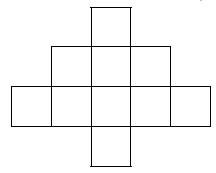
\includegraphics[scale=0.35]{166.png}}
\end{figure}
\end{center}
224. Расставьте в клетках фигуры числа от 1 до 10, каждое по одному разу, так, чтобы в любой полоске из трёх клеток (горизонтальной или вертикальной) сумма делилась на 3.
\begin{center}
\begin{figure}[ht!]
\center{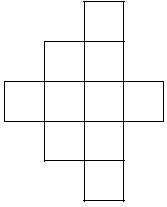
\includegraphics[scale=0.35]{16.png}}
\end{figure}
\end{center}
225. На клетчатой бумаге поставлены точки. Соедините их отрезками таким образом, чтобы каждая точка была вершиной квадрата.
\begin{center}
\begin{figure}[ht!]
\center{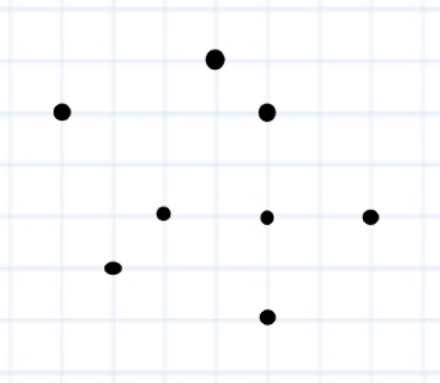
\includegraphics[scale=0.3]{01.png}}
\end{figure}
\end{center}
226. У Винтика и Шпунтика на 4 коробках были таблички <<Гайки и отвёртки>>, <<Молотки>>, <<Отвёртки>>, <<Гайки и молотки>>. Незнайка случайно перепутал таблички так, что ни в одной из коробок не лежит ничего из того, что упомянуто на табличке. Что лежит в коробке с надписью <<Отвёртки>>?\\
227. На гранях кубика написаны 6 натуральных чисел, три из которых видны на рисунке. Известно, что произведение чисел, написанных на противоположных гранях, одинаковы. Какое наименьшее значение может принимать сумма всех чисел на гранях кубика?
\begin{center}
\begin{figure}[ht!]
\center{\includegraphics[scale=0.25]{02.png}}
\end{figure}
\end{center}
228. Запишите наибольшее шестизначное число, для которого выполняются все следующие условия:\\
1) все цифры этого числа различны;\\
2) если умножить любую из его цифр на цифру, стоящую в разряде десятков, в результате будет одно и то же число;\\
3) первая и третья цифра делятся на вторую цифру.\\
229. Запишите наименьшее шестизначное число, для которого выполняются все следующие условия:\\
1) все цифры этого числа различны;\\
2) если умножить любую из его цифр на цифру, стоящую в разряде сотен, в результате будет одно и то же число;\\
3) третья и пятая цифра делятся на шестую цифру.\\
230. Сколько существует пятизначных чисел с суммой цифр три?\\
231. Сколько существует четырёхзначных чисел с суммой цифр четыре?\\
232. Кузнечик прыгает по клеточной полоске двумя способами: первым $(1)$ --- вперёд на пять клеток, вторым $(2)$ --- назад на три клетки. При этом он красит в чёрный цвет каждую клетку,  в которой он побывал. Запишите последовательности команд, благодаря которой он покрасит только клетки с первой по 10. Он начинает в клетке с номером 1.\\
233. Кузнечик прыгает по клеточной полоске двумя способами: первым $(1)$ --- вперёд на семь клеток, вторым $(2)$ --- назад на четыре клетки. При этом он красит в чёрный цвет каждую клетку в которой он побывал. Запишите последовательности команд, благодаря которой он покрасит только клетки с первой по четырнадцатую. Он начинает в клетке с номером 1.\\
234. На острове живут рыцари и лжецы. Путник встретил троих островитян и спросил каждого из них: <<Сколько рыцарей среди твоих спутников?>>. Первый сказал --- <<ни одного>>,  второй сказал --- <<один>>. Что сказал третий?\\
235. На острове живут рыцари и лжецы. Путник встретил троих островитян и спросил каждого из них: <<Сколько рыцарей среди твоих спутников?>>. Первый сказал --- <<один>>,  второй сказал --- <<ни одного>>. Что сказал третий?\\
236. Нарисуйте несколько прямоугольников так, чтобы все внутренние части оказались треугольниками, и их было не меньше шести.\\
237. Паша построил четырёхуровневую пирамиду, так что каждый кубик опирается на четыре других нижних кубика. Саша хочет увеличить пирамиду в высоту на два этажа. Сколько кубиков ему потребуется?\\
238. С полудня до полуночи Кот Учёный спит под дубом, а с полуночи до полудня рассказывает сказки. Кот повесил на дубе плакат: <<Через час я буду делать то же самое, что делал два часа назад>>. Сколько часов в сутки эта надпись верна?\\
239. С полудня до полуночи Кот Учёный спит под дубом, а с полуночи до полудня рассказывает сказки. Кот повесил на дубе плакат: <<Через два часа я буду делать то же самое, что делал три часа назад>>. Сколько часов в сутки эта надпись верна?\\
240. Имеются три гири 1кг, 2кг, 9кг. Какие веса можно взвесить с помощью этих гирь на весах с двумя чашами, если можно класть гири на обе чаши? Перечислите все варианты в порядке возрастания.\\
241. Имеются три гири 1кг, 2кг, 10кг. Какие веса можно взвесить с помощью этих гирь на весах с двумя чашами, если можно класть гири на обе чаши? Перечислите все варианты в порядке возрастания.\\
242. Сколько существует натуральных чисел $N$ таких, что ровно два из трёх чисел $N, N+10, N+25$ являются трёхзначными?\\
243. Сколько существует натуральных чисел $N$ таких, что ровно два из трёх чисел $N, N+15, N+20$ являются трёхзначными?\\
244. Число называется палиндромом, если оно читается слева направо и справа налево одинаково (например, 1221 и 15651 --- палиндромы). Будем называть число {\bf красивым}, если числа, большие его на 3 и на 5, оба являются палиндромами. Придумайте какое-нибудь красивое четырёхзначное число.\\
245. Число называется палиндромом, если оно читается слева направо и справа налево одинаково (например, 1221 и 15651 --- палиндромы). Будем называть число {\bf красивым}, если числа, меньшие его на 3 и на 5, оба являются палиндромами. Придумайте какое-нибудь красивое четырёхзначное число.\\
246. Про четырёхзначное число известно, что сумма его цифр равна разности 2019 и самого числа. Найдите все такие числа.\\
247. Про четырёхзначное число известно, что сумма его цифр равна разности 2021 и самого числа. Найдите все такие числа.\\
248. Сумма 15 натуральных чисел равна 18. Чему может быть равно произведение?\\
249. Сумма 16 натуральных чисел равна 19. Чему может быть равно произведение?\\
250. Найдите все решения ребуса ДУБ+ДУБ+ДУБ=БББ+36. (Одинаковые буквы означают одинаковые цифры, разные буквы --- разные цифры.)\\
251. Найдите все решения ребуса МЯУ+МЯУ+МЯУ=УУУ+48. (Одинаковые буквы означают одинаковые цифры, разные буквы --- разные цифры.)\\
252. По кругу стоят 30 детей. Дед Мороз дарит им подарки: первому 1, второму 2, следующему 1, потом 2 и так далее. Всего он подарил 55 подарков (пока не кончились подарки). Сколько детей получили ровно 2 подарка?\\
253. По кругу стоят 32 ребёнка. Дед Мороз дарит им подарки: первому 4, второму 2, следующему 4, потом 2 и так далее. Всего он подарил 112 подарков (пока не кончились подарки). Сколько детей получили ровно 4 подарка?\\
254. На рисунке показана полоска $2\times 8,$ её периметр равен 20. Если удалить клетки A и C или B и C, то она развалится на части, а если удалить клетки A и B, то периметр оставшейся части станет равен 22. Сколько есть способов удалить из полоски $2\times 20$ две клетки так, чтобы она осталась целой, а периметр оставшейся части был равен 48?
\begin{figure}[ht!]
\center{\includegraphics[scale=0.35]{05.png}}
\end{figure}\\
255. На рисунке показана полоска $2\times 8,$ её периметр равен 20. Если удалить клетки A и C или B и C, то она развалится на части, а если удалить клетки A и B, то периметр оставшейся части станет равен 22. Сколько есть способов удалить из полоски $2\times 21$ две клетки так, чтобы она осталась целой, а периметр оставшейся части был равен 50?
\begin{figure}[ht!]
\center{\includegraphics[scale=0.35]{05.png}}
\end{figure}\\
256. Аня посчитала сумму всех трёхзначных чисел, оканчивающихся на 9, Вася вычислил сумму всех трёхзначных чисел, последняя цифра которых 8. Саша нашёл сумму всех трёхзначных чисел, оканчивающихся на 4, а Дима сложил все трёхзначные числа, оканчивающиеся двойкой. Аня и Саша сложили свои результаты, а Вася и Дима --- свои. У кого сумма оказалась больше? На сколько?\\
257. Аня посчитала сумму всех трёхзначных чисел, оканчивающихся на 8, Вася вычислил сумму всех трёхзначных чисел, последняя цифра которых 9. Саша нашёл сумму всех трёхзначных чисел, оканчивающихся на 4, а Дима сложил все трёхзначные числа, оканчивающиеся двойкой. Аня и Саша сложили свои результаты, а Вася и Дима --- свои. У кого сумма оказалась больше? На сколько?\\
258. У какого числа от 2381895 до 2761984 самая большая сумма цифр?\\
259. У какого числа от 3497029 до 3813472 самая большая сумма цифр?\\
260. Придумайте три числа с суммой 83, произведение которых заканчивается на 4 нуля.\\
261. Придумайте три числа с суммой 91, произведение которых заканчивается на 4 нуля.
ewpage
oindent
262. \begin{figure}[ht!]
\center{\includegraphics[scale=0.3]{rss.png}}
\end{figure}\\
На рисунке показан прямоугольник $2\times4.$ Если удалить клетки $A$ и $C$ или $B$ и $C,$ то он развалится на две части, а если удалить клетки $A$ и $B,$ то не развалится. А какое наименьшее количество клеток в прямоугольнике $5\times7$ нужно удалить, чтобы он развалился на части?\\
263. \begin{figure}[ht!]
\center{\includegraphics[scale=0.3]{rss.png}}
\end{figure}\\
На рисунке показан прямоугольник $2\times4.$Если удалить клетки $A$ и $C$ или $B$ и $C,$ то он развалится на две части, а если удалить клетки $A$ и $B,$ то не развалится. А какое наименьшее количество клеток в прямоугольнике $5\times6$ нужно удалить, чтобы он развалился на части?\\
264. У нечётного четырёхзначного числа вычислили сумму его последней цифры и трёхзначного числа, получаемого вычёркиванием последней цифры из данного. Получилось 203. Каким могло быть исходное четырёхзначное число?\\
265. У чётного четырёхзначного числа вычислили сумму его последней цифры и трёхзначного числа, получаемого вычёркиванием последней цифры из данного. Получилось 204. Каким могло быть исходное четырёхзначное число?\\
266. В последовательности $1, 2, 2, 4, 8, 2, 6, \ldots$ каждая цифра равна последней цифре произведения предыдущих двух цифр. Как видно, на 4-м месте стоит цифра 4. А какая цифра стоит на 2021-м месте?\\
267. В последовательности $2, 1, 2, 2, 4, 8, 2, \ldots$ каждая цифра равна последней цифре произведения предыдущих двух цифр. Как видно, на 6-м месте стоит цифра 8. А какая цифра стоит на 2021-м месте?\\
268. На электронных часах высвечивается $11:13:33.$ Через какое время впервые пять из шести цифр на табло часов окажутся одинаковыми?\\
269. На электронных часах высвечивается $11:14:44.$ Через какое время впервые пять из шести цифр на табло часов окажутся одинаковыми?\\
270. Если из квадрата $3\times3$ вырезать центральную клетку, то в нём будет 8 внутренних перегородок. Если же из квадрата $4\times4$ вырезать дырку $2\times2,$ то будет 12 внутренних перегородок. Из прямоугольника $100\times200$ вырезали две непересекающиеся и несоприкасающиеся квадратные дырки $7\times7.$ Сколько осталось внутренних перегородок?\\
271. Если из квадрата $3\times3$ вырезать центральную клетку, то в нём будет 8 внутренних перегородок. Если же из квадрата $4\times4$ вырезать дырку $2\times2,$ то будет 12 внутренних перегородок. Из прямоугольника $100\times200$ вырезали две непересекающиеся и несоприкасающиеся квадратные дырки $8\times8.$ Сколько осталось внутренних перегородок?\\
272. В углу прямоугольника $3\times5$ стоит кубик (размер грани кубика совпадает с клеткой). У данного кубика сильно испачкана одна грань. Можно перекатывать кубик через ребро, при этом запрещено выкатывать его за пределы прямоугольника и ставить на клетку, на которой кубик уже стоял. Придумайте способ испачкать как можно больше клеток прямоугольника. Какая именно грань кубика запачкана, вы можете выбрать сами. В каждой клетке прямоугольника запишите, какой по счёту эта клетка окажется под кубиком (в клетке, на которой кубик стоит изначально, запишите число 1). В ответ запишите число испачканных клеток.
\begin{center}
\begin{figure}[ht!]
\center{\includegraphics[scale=0.35]{kub1.png}}
\end{figure}
\end{center}
273. В углу прямоугольника $3\times6$ стоит кубик (размер грани кубика совпадает с клеткой). У данного кубика сильно испачкана одна грань. Можно перекатывать кубик через ребро, при этом запрещено выкатывать его за пределы прямоугольника и ставить на клетку, на которой кубик уже стоял. Придумайте способ испачкать как можно больше клеток прямоугольника. Какая именно грань кубика запачкана, вы можете выбрать сами. В каждой клетке прямоугольника запишите, какой по счёту эта клетка окажется под кубиком (в клетке, на которой кубик стоит изначально, запишите число 1). В ответ запишите число испачканных клеток.
\begin{center}
\begin{figure}[ht!]
\center{\includegraphics[scale=0.35]{kub2.png}}
\end{figure}
\end{center}
274. Муравьишка ползёт по поверхности кубика (вертикально или горизонтально) из точки $A$ в точку $B$ по пути, отмеченному стрелками. Чему равна длина этого пути, если ребро кубика равно 15 см?
\begin{center}
\begin{figure}[ht!]
\center{\includegraphics[scale=0.35]{mur.png}}
\end{figure}
\end{center}
275. \begin{center}
\begin{figure}[ht!]
\center{\includegraphics[scale=0.35]{treug.png}}
\end{figure}
\end{center}
Сколько клеточек составляет площадь фигуры?\\
276. Винни Пух и Пятачок проверяют запасы мёда у Кролика. Они подсчитали, что у Кролика всего 7 горшочков цветочного мёда, 6 горшочков липового мёда и 3 горшочка гречишного мёда. Увлёкшись проверкой, Винни Пух съел 2 горшочка мёда. Что могло при этом получиться? ({\it выберите один или несколько возможных вариантов})\\
1. У Кролика не осталось гречишного мёда.\\
2. Горшочков липового мёда стало меньше, чем гречишного.\\
3. Горшочков всех видов мёда стало поровну.\\
4. Горшочков двух видов мёда стало поровну.\\
5. Горшочков с цветочным мёдом стало больше, чем всех остальных вместе.\\
6. Горшочков какого-то вида мёда стало ровно половина от всех оставшихся горшочков мёда.
ewpage
oindent
277. \begin{center}
\begin{figure}[ht!]
\center{\includegraphics[scale=0.35]{pol.png}}
\end{figure}
\end{center}
На полу лежат четыре прямоугольных ковра, перекрывая друг друга. Напишите номера всех областей, которые покрыты ровно тремя из них.
ewpage
oindent
278. \begin{center}
\begin{figure}[ht!]
\center{\includegraphics[scale=0.35]{giri.png}}
\end{figure}
\end{center}
С гирьками проделали 3 взвешивания. Какая гирька самая тяжёлая и какая самая лёгкая?\\
279. Ёжик загадал четырёхзначное число $A,$ все цифры которого различны, а Крош его угадывает. Крош уже узнал, что:\\
 --- число 8702 содержит ровно одну цифру числа $A,$ причём на правильном месте;\\
 --- число 8237 содержит ровно две цифры числа $A,$ причём одна на правильном месте, а вторая на неправильном месте;\\
 --- число 7024 содержит ровно одну цифру числа $A,$ причём на правильном месте;\\
 --- число 7130 содержит ровно две цифры числа $A,$ причём обе на неправильных местах.\\
 Какое число загадал Ёжик?\\
  {\it {\textbf {Запишите только ответ, пояснять его не нужно.}}}\\
280. Робот Федя ходит по клетчатому полю. Каждый раз после перехода в соседнюю клетку Федя поворачивает налево или направо. Поворот налево занимает у него 5 секунд, а поворот направо --- 3 секунды. После этого 7 секунд он идёт до следующего поворота. Он начал своё движение с поворота налево и закончил перед поворотом. После старта Федя путешествовал по полю 2 минуты и 2 секунды. Сколько раз он при этом мог поворачивать направо? {\textbf {Найдите все возможные варианты.}}\\
281. Найдите какое-нибудь натуральное число, которое делится на 12, 35 и 15 одновременно.\\
282. Найдите какое-нибудь натуральное число, которое делится на 6, 8, 9 и 21 одновременно.\\
283. Нарисуйте 5 отрезков так, чтобы можно было закрасить (внутри) синим цветом 5 треугольников и красным один пятиугольник. На плоскости не должно быть точек двух цветов сразу. Отметьте точками или буквами начала и концы отрезков.\\
284. Нарисуйте на плоскости 7 отрезков так, чтобы можно было закрасить (внутри) синим цветом 2 квадрата и красным один пятиугольник. На плоскости не должно быть точек двух цветов сразу. Отметьте точками или буквами начала и концы отрезков.\\
285. Анатолий выписал на доску все двузначные числа, делящиеся на 4. Сколько раз он написал цифру 6?\\
286. Петя выписал на доску все двузначные числа, делящиеся на 4. Сколько раз он написал цифру 8?\\
287. От прямоугольника отрезали с двух противоположных сторон по квадрату, так чтобы эти квадраты не имели общих сторон. В результате получился прямоугольник с периметром на 24 меньше. Найдите периметр каждого квадрата.\\
288. От прямоугольника отрезали с двух противоположных сторон по квадрату, так чтобы эти квадраты не имели общих сторон. В результате получился прямоугольник с периметром на 36 меньше. Найдите периметр каждого квадрата.\\
289. Вчера было 15.05 и номер дня был ровно в три раза больше номера месяца. Сколько таких дней в 2021 году?\\
290. Скоро будет 20.05 и номер дня будет ровно в четыре раза больше номера месяца. Сколько таких дней в 2021 году?\\
291. Саша по вторникам и субботам называет числа правильно, по понедельникам и пятницам преувеличивает числа в 3 раза, а в остальные дни уменьшает числа на 1. Он шесть дней подряд отвечал на вопрос <<Какого числа ты родился?>> Мог ли он назвать числа 2, 3, 3, 3, 9, 9 в каком-то порядке? Если да --- покажите как, если нет --- объясните почему.\\
292. Представьте число 2547 в виде суммы трёх трёхзначных чисел таких, что в их записи все 9 цифр были бы различны.\\
293. Представьте число 2543 в виде суммы трёх трёхзначных чисел таких, что в их записи все 9 цифр были бы различны.\\
294. Сколько существует пятизначных чисел, в записи каждого из которых есть цифра 5 или цифра 7?\\
295. Сколько существует пятизначных чисел, в записи каждого из которых есть цифра 2 или цифра 4?\\
296. У четырёхзначного числа вычислили сумму его последней цифры и трёхзначного числа, получаемого вычёркиванием предпоследней цифры из данного. Получилось 204. Каким могло быть исходное четырёхзначное число? Выберите из них то, у которого наибольшая сумма цифр и запишите его в ответ.\\
297. У четырёхзначного числа вычислили сумму его последней цифры и трёхзначного числа, получаемого вычёркиванием предпоследней цифры из данного. Получилось 206. Каким могло быть исходное четырёхзначное число? Выберите из них то, у которого наибольшая сумма цифр и запишите его в ответ.\\
298. На электронных часах высвечивается $11:30:00.$ Какое время назад последний раз пять из шести цифр на табло часов были одинаковыми?\\
299. На электронных часах высвечивается $22:40:00.$ Какое время назад последний раз пять из шести цифр на табло часов были одинаковыми?\\
300. Если из квадрата $3\times3$ вырезать центральную клетку, то в нём будет 8 внутренних перегородок. Если же из квадрата $4\times4$ вырезать дырку $2\times2,$ то будет 12 внутренних перегородок. Из квадрата вырезали пять непересекающихся и не соприкасающихся дырок $2\times2.$ В полученной фигуре оказалось ровно 20952 внутренних перегородки. Чему равна сторона квадрата?\\
301. Если из квадрата $3\times3$ вырезать центральную клетку, то в нём будет 8 внутренних перегородок. Если же из квадрата $4\times4$ вырезать дырку $2\times2,$ то будет 12 внутренних перегородок. Из квадрата вырезали пять непересекающихся и не соприкасающихся дырок $2\times2.$ В полученной фигуре оказалось ровно 21364 внутренних перегородки. Чему равна сторона квадрата?\\
302. Каждый четвероклассник пожал руку четырём пятиклассникам и шести четвероклассникам, при этом каждый пятиклассник пожал руку шести четвероклассникам и семи пятиклассникам. Сколько четвероклассников, если всего в двух классах 50 человек?\\
303. Каждый четвероклассник пожал руку трём пятиклассникам и шести четвероклассникам, при этом каждый пятиклассник пожал руку семи четвероклассникам и пяти пятиклассникам. Сколько пятиклассников, если всего в двух классах 50 человек?\\
304. \begin{figure}[ht!]
\center{\includegraphics[scale=0.35]{tab.png}}
\end{figure}\\
Расставьте в каждую клетку таблицы $3\times6$ букву К, А или С так, чтобы у каждой К было 4 соседа А, а у каждой С было ровно два соседа А, а у каждой А среди соседей есть и К, и С. Соседи считаются только по стороне.\\
305. \begin{figure}[ht!]
\center{\includegraphics[scale=0.35]{tab.png}}
\end{figure}\\
Расставьте в каждую клетку таблицы $3\times6$ букву М, Я или П так, чтобы у каждой М было 4 соседа Я, а у каждой П было ровно два соседа Я, а у каждой Я среди соседей есть и М, и П. Соседи считаются только по стороне.\\
306. На схеме изображён пустой стальной кубик со стороной 1 метр. На каждой его грани нарисовали 25 одинаковых квадратиков и просверлили три дырки как показано на рисунке. Кубик можно ставить на другие грани, но нельзя дыркой вниз. Какое наибольшее количество литров воды можно налить в этот кубик? Напомним, что литр --- это дециметр кубический.
\begin{figure}[ht!]
\center{\includegraphics[scale=0.35]{kub.png}}
\end{figure}\\
307. На схеме изображён пустой стальной кубик со стороной 1 метр. На каждой его грани нарисовали 25 одинаковых квадратиков и просверлили три дырки как показано на рисунке. Кубик можно ставить на другие грани, но нельзя дыркой вниз. Какое наибольшее количество литров воды можно налить в этот кубик? Напомним, что литр --- это дециметр кубический.
\begin{figure}[ht!]
\center{\includegraphics[scale=0.35]{kukub.png}}
\end{figure}\\
308. На рисунке изображены углы. Запишите в ответ номера углов в следующем порядке: острый, прямой, тупой.\\
\begin{figure}[ht!]
\center{\includegraphics[scale=0.35]{ugl2.png}}
\end{figure}
ewpage
oindent
309. На рисунке изображены углы. Запишите в ответ номера углов в следующем порядке: острый, прямой, тупой.\\
\begin{figure}[ht!]
\center{\includegraphics[scale=0.35]{ugl1.png}}
\end{figure}\\
310. На трёх непрозрачных банках написано: {\bf <<Горох>>; <<Не горох>>; <<Горох или пуговицы>>.} Известно, что все эти надписи ложны. При этом в банках лежат горох, мука и пуговицы. В которой из банок лежит мука?\\
311. На трёх непрозрачных банках написано: {\bf <<Крупа>>; <<Не крупа>>; <<Крупа или гайки>>.} Известно, что все эти надписи ложны. При этом в банках лежат крупа, сахар и гайки. В которой из банок лежит сахар?\\
312. Отрезки $AB,\ BC$ и $CK$ расположены на одной прямой, причём точка $C$ лежит между точками $A$ и $B,$ а точка $B$ между точками $C$ и $K.$Чему равна длина отрезка $AK,$ если $AB=10$ см, $BC=3$ см, $CK=8$ см?\\
313. Отрезки $MP,\ PK$ и $KA$ расположены на одной прямой, причём точка $K$ лежит между точками $M$ и $P,$ а точка $P$ между точками $A$ и $K.$Чему равна длина отрезка $AM,$ если $MP=12$ см, $PK=2$ см, $KA=6$ см?\\
314. Дано число 29546381. Вычеркните в нём три цифры так, чтобы оставшееся число было наибольшим чётным. Результат запишите.\\
315. Дано число 29546318. Вычеркните в нём три цифры так, чтобы оставшееся число было наименьшим нечётным. Результат запишите.\\
316. Найдите периметр самого большого прямоугольника на рисунке, если площадь закрашенного квадрата равна $64\text{ см}^2.$ Все 5 фигур, из которых составлен большой прямоугольник --- квадраты.\\
\begin{figure}[ht!]
\center{\includegraphics[scale=0.35]{pram1.png}}
\end{figure}\\
317. Найдите периметр самого большого прямоугольника на рисунке, если площадь закрашенного квадрата равна $16\text{ см}^2.$ Все 5 фигур, из которых составлен большой прямоугольник --- квадраты.\\
\begin{figure}[ht!]
\center{\includegraphics[scale=0.35]{pram2.png}}
\end{figure}\\
318. Для двух групп экскурсантов заказали 472 конфеты и 118 бутербродов. Количество людей в группах отличается не более, чем на 2. В каждой группе меньше 35 людей. Сколько людей в каждой группе, если ни один человек не получит ни конфет, ни бутербродов больше, чем другой? Если в группах разное количество людей, запишите в ответ меньшее число.\\
319. Для двух групп экскурсантов заказали 427 конфет и 122 бутерброда. Количество людей в группах отличается не более, чем на 2. В каждой группе меньше 35 людей. Сколько людей в каждой группе, если ни один человек не получит ни конфет, ни бутербродов больше, чем другой? Если в группах разное количество людей, запишите в ответ большее число.\\
320. Замените звёздочки цифрами так, чтобы равенство стало верным и все семь цифр были различными: $**+**=175.$\\
321. Замените звёздочки цифрами так, чтобы равенство стало верным и все семь цифр были различными: $**+**=176.$\\
322. Серёжа согнул две проволоки так, как показано на рисунке, и наложил их друг на друга, не разгибая. Какова наибольшая возможная длина их общей (совпавшей) части, если 2 клеточки равны 1 см?\\
\begin{figure}[ht!]
\center{\includegraphics[scale=0.35]{prov1.png}}
\end{figure}\\
323. Серёжа согнул две проволоки так, как показано на рисунке, и наложил их друг на друга, не разгибая. Какова наибольшая возможная длина их общей (совпавшей) части, если 1 клеточка равна 1 см?\\
\begin{figure}[ht!]
\center{\includegraphics[scale=0.35]{prov2.png}}
\end{figure}\\
324. У Кроша есть шесть карточек, на которых записаны числа 415, 41, 7, 19, 78, 3. Расположите карточки в ряд так, чтобы получившееся одиннадцатизначное число было наименьшим из возможных.\\
325. У Кроша есть шесть карточек, на которых записаны числа 435, 43, 7, 13, 74, 3. Расположите карточки в ряд так, чтобы получившееся одиннадцатизначное число было наименьшим из возможных.\\
326. Отрезок, равный 28 см, разделён на три (возможно, неравных) отрезка. Расстояние между серединами крайних отрезков равно 16 см. Найдите длину среднего отрезка.\\
327. Отрезок, равный 30 см, разделён на три (возможно, неравных) отрезка. Расстояние между серединами крайних отрезков равно 16 см. Найдите длину среднего отрезка.\\
328. Перед Вами марсианская единица измерения площади --- шкрындла. Измерьте приведённые ниже фигуры в
шкрындлах.\\
\begin{figure}[ht!]
\center{\includegraphics[scale=0.35]{sc1.png}}
\end{figure}\\
329. Перед Вами марсианская единица измерения площади --- шкрындла. Измерьте приведённые ниже фигуры в
шкрындлах.\\
\begin{figure}[ht!]
\center{\includegraphics[scale=0.35]{sc2.png}}
\end{figure}\\
330. Чему равняется сумма цифр числа $1\underbrace{00\ldots00}_{2022}-2022?$\\
331. Чему равняется сумма цифр числа $1\underbrace{00\ldots00}_{2021}-2021?$\\
332. Петя посчитал сумму первой тысячи натуральных чисел, делящихся на 6. А Вася посчитал сумму первой тысячи нечётных натуральных чисел, делящихся на 3. Найдите разность чисел, получившихся у мальчиков.\\
333. Петя посчитал сумму первой тысячи натуральных чисел, делящихся на 10. А Вася посчитал сумму первой тысячи нечётных натуральных чисел, делящихся на 5. Найдите разность чисел, получившихся у мальчиков.\\
334. Крош и Бараш в $9:00$ одновременно вышли друг к другу в гости. Каждый из них идёт с постоянной скоростью. Через полчаса они встретились в первый раз, поздоровались и пошли дальше. Добравшись до домика друг друга и убедившись, что там никого нет, оба повернули обратно. Во сколько Крош и Бараш встретятся второй раз?\\
335. Крош и Бараш в $10:00$ одновременно вышли друг к другу в гости. Каждый из них идёт с постоянной скоростью. Через час они встретились в первый раз, поздоровались и пошли дальше. Добравшись до домика друг друга и убедившись, что там никого нет, оба повернули обратно. Во сколько Крош и Бараш встретятся второй раз?\\
336. На доске написано трёхзначное число. Петя поменял в нём первую и последнюю цифру местами и написал полученное число на доске. Оказалось, что разница написанных чисел --- это трёхзначное число. Найдите вторую цифру разницы написанных чисел.\\
337. В примере на сложение $\star54\star\star+\star82\star\star=10\star793$ звёздочками заменены некоторые цифры (не обязательно одинаковые). Найдите сумму этих семи цифр.\\
338. В примере на сложение $\star62\star\star+\star73\star\star=11\star691$ звёздочками заменены некоторые цифры (не обязательно одинаковые). Найдите сумму этих семи цифр.\\
339. Придумайте три различных трёхзначных числа с суммой 817, которые отличаются только первой цифрой. В ответ запишите все три числа.\\
340. Придумайте три различных трёхзначных числа с суммой 917, которые отличаются только первой цифрой. В ответ запишите все три числа.\\
341. Сколько существует пятизначных чисел, в записи каждого из которых первая цифра больше третьей?\\
342. Сколько существует пятизначных чисел, в записи каждого из которых первая цифра больше четвёртой?\\
343. В углу квадрата $2025\times2025$ живёт жук, а в противоположном углу этого квадрата находится его школа. Жук умеет за один шаг переходить в соседний по стороне или вершине квадратик. Тем самым, чтобы добраться до школы, ему надо сделать 2024 шага. В некоторый момент в центральном квадратике $1\times1$ случилась авария, и теперь ему до школы 2024 шага. Сколько шагов надо будет сделать жуку до школы, если авария разрастётся до квадрата $7\times7$ (центры аварии и большого квадрата совпадают)?\\
344. В углу квадрата $2023\times2023$ живёт жук, а в противоположном углу этого квадрата находится его школа. Жук умеет за один шаг переходить в соседний по стороне или вершине квадратик. Тем самым, чтобы добраться до школы, ему надо сделать 2022 шага. В некоторый момент в центральном квадратике $1\times1$ случилась авария, и теперь ему до школы 2023 шага. Сколько шагов надо будет сделать жуку до школы, если авария разрастётся до квадрата $7\times7$ (центры аварии и большого квадрата совпадают)?
ewpage
oindent
345. На квадратном поле $4\times4$ клетки растут цветы, число цветов в каждой клетке указано на схеме. Вася начинает с левой нижней клетки (с числом 8) и, переходя каждый раз в соседнюю справа или сверху, добирается до правой верхней клетки, собирая цветы с клеток, на которых побывал. Сколько есть маршрутов, на которых Вася соберёт ровно 25 цветков?\\
\begin{figure}[ht!]
\center{\includegraphics[scale=0.35]{flow1.png}}
\end{figure}\\
346. На квадратном поле $4\times4$ клетки растут цветы, число цветов в каждой клетке указано на схеме. Вася начинает с левой нижней клетки (с числом 2) и, переходя каждый раз в соседнюю справа или сверху, добирается до правой верхней клетки, собирая цветы с клеток, на которых побывал. Сколько есть маршрутов, на которых Вася соберёт ровно 43 цветка?\\
\begin{figure}[ht!]
\center{\includegraphics[scale=0.35]{flow2.png}}
\end{figure}\\
347. На электронном табло высвечивается время $23:23:23.$ В какое время после этого в шестой раз все цифры на табло будут различными?\\
348. На электронном табло высвечивается время $12:12:12.$ В какое время после этого в седьмой раз все цифры на табло будут различными?\\
349. Алексей, Борис, Виктор и Георгий играли в игры, ничьих не было. По итогам они частично заполнили таблицу, кто сколько раз у кого выиграл. Если в клетке на пересечении строки Алексея и столбца Виктора написано $2:1,$ это значит, что Алексей выиграл у Виктора 2 раза и 1 раз ему проиграл. Известно, что Георгий проиграл в три раза больше раз, чем выиграл; Борис выиграл пять раз; Виктор проиграл Георгию четверть от всех игр между ними; Алексей проиграл каждому одинаковое число раз. Сколько раз Алексей выиграл у Георгия? Заполните целиком таблицу ниже.\\
\begin{figure}[ht!]
\center{\includegraphics[scale=0.35]{tab3.png}}
\end{figure}
ewpage
oindent
350. Борис, Виктор, Георгий и Дмитрий играли в игры, ничьих не было. По итогам они частично заполнили таблицу, кто сколько раз у кого выиграл. Если в клетке на пересечении строки Дмитрия и столбца Виктора написано $2:1,$ это значит, что Дмитрий выиграл у Виктора 2 раза и 1 раз ему проиграл. Известно, что Дмитрий проиграл в три раза больше раз, чем выиграл; Виктор выиграл пять раз; Георгий проиграл Дмитрию треть от всех игр между ними; Борис проиграл каждому одинаковое число раз. Сколько раз Дмитрий проиграл Борису? Заполните целиком таблицу ниже.\\
\begin{figure}[ht!]
\center{\includegraphics[scale=0.35]{tab4.png}}
\end{figure}\\
351. При чтении числа 2002 наоборот получается точно такое же число. А какое ближайшее число к 2002 обладает таким же свойством?\\
352. При чтении числа 3003 наоборот получается точно такое же число. А какое ближайшее число
к 3003 обладает таким же свойством?\\
353. Александр Маркович положил в актовый зал квадратные ковры размерами $14 \times 14,\ 15 \times 15$ метров. Какая наименьшая площадь пола может быть покрыта сразу двумя коврами, если актовый зал имеет форму квадрата со стороной 20 метров?\\
354. Александр Маркович положил в актовый зал квадратные ковры размерами $14 \times 14,\ 15 \times 15$ метров. Какая наименьшая площадь пола может быть покрыта сразу двумя коврами, если актовый зал имеет форму квадрата со стороной 19 метров?\\
355. Найдите самое большое 10-значное число, в котором все цифры различны и любые две соседние цифры отличаются хотя бы на 2.\\
356. Найдите самое маленькое 10-значное число, в котором все цифры различны и любые две соседние цифры отличаются хотя бы на 2.\\
357. У Пети есть 4 красных, 7 зелёных, 8 синих, 10 белых и 11 чёрных шариков. Какое минимальное число шариков надо перекрасить в другой цвет так, чтобы шариков каждого из пяти цветов было поровну?\\
358. У Пети есть 3 красных, 7 зелёных, 9 синих, 10 белых и 11 чёрных шариков. Какое минимальное число шариков надо перекрасить в другой цвет так, чтобы шариков каждого из пяти цветов было поровну?\\
359. Какие две цифры можно зачеркнуть в данном выражении так, чтобы получить верное математическое равенство? Найдите все варианты. (Записи 36/12 и 84/12 означают деление.)
$$ 36/12+5=84/12+4.$$
360. Какие две цифры можно зачеркнуть в данном выражении так, чтобы получить верное математическое равенство? Найдите все варианты. (Записи 48/12 и 72/12 означают деление.)
$$48/12+3=72/12+5.$$
361. Чему равна сумма цифр числа $\underbrace{99\ldots99}_{100}+2023?$\\
362. Чему равна сумма цифр числа $\underbrace{99\ldots99}_{100}+2024?$\\
363. Маша, Ксюша, Соня и Даша сыграли вместе 6 партий в теннис. В каждой игре они вчетвером делились на две команды по два человека, и одна из команд выигрывала игру. Маша была в команде-победительнице 5 раз, Ксюша --- 2 раза, а Соня --- 1 раз. А сколько раз Даша была в команде-победительнице?\\
364. Маша, Ксюша, Соня и Даша сыграли вместе 6 партий в теннис. В каждой игре они вчетвером делились на две команды по два человека, и одна из команд выигрывала игру. Маша была в команде-победительнице 4 раза, Ксюша --- 3 раза, а Соня --- 2 раза. А сколько раз Даша была в команде-победительнице?\\
365. Добавьте к записи числа 8072 три цифры (в любые места --- впереди, сзади, между цифрами) так, чтобы получившееся число было нечётным, все его цифры были различны, и оно было наибольшим из таких чисел. Запишите это число.\\
366. Добавьте к записи числа 2079 три цифры (в любые места --- впереди, сзади, между цифрами) так, чтобы получившееся число было чётным, все его цифры были различны, и оно было наименьшим из таких чисел. Запишите это число.\\
367. В записи двух трёхзначных чисел использованы только чётные цифры, причём повторяется только одна из них. Чему равна сумма произведения всех этих цифр
и наибольшего двузначного числа?\\
368. В записи трёх двузначных чисел использованы только чётные цифры, причём повторяется только одна из них. Чему равна разность наименьшего
трёхзначного числа и произведения всех цифр этих двузначных чисел?\\
369. Юра обещал вымыть пол или выучить песню. Выберите набор (или наборы) действий, при котором он не выполнит обещание.\\
А. вымоет пол, покормит кошку;  \qquad \qquad Б. покормит кошку, вымоет посуду;\\
В. покормит кошку, выучит песню; \qquad \quad Г. выучит песню, вымоет пол.\\
370. Ксюша обещала вымыть посуду или решить пример. Выберите набор (или наборы) действий, при котором она не выполнит обещание.\\
А. вымоет посуду, погуляет с собакой;  \qquad \quad Б. покормит кошку, решит пример;\\
В. погуляет с собакой, покормит кошку; \qquad  Г. решит пример, вымоет посуду.\\
371. \begin{figure}[ht!]
\center{\includegraphics[scale=0.35]{usl1.png}}
\end{figure}\\
372. \begin{figure}[ht!]
\center{\includegraphics[scale=0.35]{usl2.png}}
\end{figure}\\
373. Какое наибольшее число, делящееся и на 5, и на 2, можно получить из числа 6032005, если
вычеркнуть ровно 3 любые цифры?\\
374. Какое наибольшее число, делящееся и на 2, и на 5, можно получить из числа 7002405, если
вычеркнуть ровно 3 любые цифры?\\
375. В некоторой стране выпустили монеты номиналами 1, 5, 10 рублей, на обратной стороне которых
могут быть изображены корона, замок или орёл. Затем все рублёвые и пятирублёвые монеты с
изображением короны вывели из обращения. На столе лежат 6 монет, как показано на картинке.
Отметьте галочкой, какие монеты обязательно нужно перевернуть, чтобы узнать, есть ли среди них
выведенные из обращения.\\
\begin{figure}[ht!]
\center{\includegraphics[scale=0.35]{mon1.png}}
\end{figure}\\
376. В некоторой стране выпустили монеты номиналами 1, 5, 10 рублей, на обратной стороне которых
могут быть изображены корона, замок или орёл. Затем все пятирублёвые и десятирублёвые монеты
с изображением замка вывели из обращения. На столе лежат 6 монет, как показано на картинке.
Отметьте галочкой, какие монеты обязательно нужно перевернуть, чтобы узнать, есть ли среди них
выведенные из обращения.\\
\begin{figure}[ht!]
\center{\includegraphics[scale=0.35]{mon1.png}}
\end{figure}\\
377. Сколько способов пройти лабиринт из точки Начало в точку Конец, если нельзя проходить по одной дороге
дважды, а также нельзя ходить справа налево?\\
\begin{figure}[ht!]
\center{\includegraphics[scale=0.35]{lab.png}}
\end{figure}\\
378. Серёже дали 5 фигурок, из которых он сложил детальку. Покажите, как он смог это сделать.
Фигурки можно крутить и переворачивать.\\
\begin{figure}[ht!]
\center{\includegraphics[scale=0.35]{fig1.png}}
\end{figure}\\
379. Серёже дали 5 фигурок, из которых он сложил детальку. Покажите, как он смог это сделать.
Фигурки можно крутить и переворачивать.\\
\begin{figure}[ht!]
\center{\includegraphics[scale=0.35]{fig2.png}}
\end{figure}\\
380.  Сегодня 21 апреля 2024 года. Запишем дату одним числом без точек и пробелов: 21042024.
Заметим, что в таком виде дата состоит из пяти частей: некое двузначное число, потом 0, потом
двузначное число в 2 раза больше предыдущего, снова 0 и затем предыдущее число с цифрами,
записанными наоборот. Сколько дат с таким свойством в XXI веке (с 2001 по 2100 год)?\\
381. Матвей может двигать фишку по клетчатой доске 36 на 39 клеток следующими способами:
1) на 1 клетку вправо и 3 клетки вверх; 2) на 2 клетки вправо; 3) на 1 вправо и на 1 вверх.
Сможет ли он такими операциями подвинуть фишку из левого нижнего угла в правый верхний?\\
382.  Матвей может двигать фишку по клетчатой доске 38 на 35 клеток следующими способами:
1) на 1 клетку влево и на 1 клетку вверх; 2) на 2 клетки влево; 3) на 1 влево и 3 вверх.
Сможет ли он такими операциями подвинуть фишку из правого нижнего угла в левый верхний?\\
383. В верном примере на сложение переставили две цифры и получилось $239+621=980.$ Запишите в ответ исходные два числа из левой части. Достаточно одного верного ответа, все искать не надо.\\
384. В верном примере на сложение переставили две цифры и получилось $771+239=930.$ Запишите в ответ исходные два числа из левой части. Достаточно одного верного ответа, все искать не надо.\\
385. Дано число 2525252. Вычёркивая из него цифры, можно получить некоторые различные четырёхзначные числа. Найдите сумму всех этих чисел.\\
386. Дано число 3434343. Вычёркивая из него цифры, можно получить некоторые различные четырёхзначные числа. Найдите сумму всех этих чисел.\\
387. По кругу по часовой стрелке ставили числа 1, 2, 3, $\ldots.$ В какой-то момент места кончились, и стали стирать старые числа и писать новые. Так, вместо числа 18 в некоторый момент написали 239, а вместо 20 написали 241. Чему будет равна сумма всех чисел сразу после того, как выпишут число 1110? Число всегда занимает одно место, даже если в нём очень много цифр.\\
388. По кругу по часовой стрелке ставили числа 1, 2, 3, $\ldots.$ В какой-то момент места кончились, и стали стирать старые числа и писать новые. Так, вместо числа 16 в некоторый момент написали 239, а вместо 18 написали 241. Чему будет равна сумма всех чисел сразу после того, как выпишут число 1111? Число всегда занимает одно место, даже если в нём очень много цифр.\\
389. В таблице $5\times5,$ клетки которой пронумерованы как на рисунке, необходимо отметить несколько клеток так, чтобы в каждой строке и в каждом столбце была отмечена ровно одна клетка. Кирилл отметил клетки с номерами 1, 13, 19 и ещё две. Чему может быть равна сумма номеров этих двух клеток?\\
\begin{figure}[ht!]
\center{\includegraphics[scale=0.35]{tab5.png}}
\end{figure}\\
390. В таблице $5\times5,$ клетки которой пронумерованы как на рисунке, необходимо отметить несколько клеток так, чтобы в каждой строке и в каждом столбце была отмечена ровно одна клетка. Кирилл отметил клетки с номерами 5, 13, 17 и ещё две. Чему может быть равна сумма номеров этих двух клеток?\\
\begin{figure}[ht!]
\center{\includegraphics[scale=0.35]{tab7.png}}
\end{figure}\\
391. В прямоугольнике $1\times2$ ровно одна перегородка, а в прямоугольнике $2\times3$ ровно 7. В прямоугольнике $105\times205$ в центре вырезали
дырку размера $15\times15.$ Сколько перегородок в получившейся фигуре?\\
392. В прямоугольнике $1\times2$ ровно одна перегородка, а в прямоугольнике $2\times3$ ровно 7. В прямоугольнике $103\times203$ в центре вырезали
дырку размера $13\times13.$ Сколько перегородок в получившейся фигуре?\\
393. В мешке лежат карандаши: белые, красные и синие (каждый цвет есть). Если вынуть 15 карандашей, то среди них обязательно будет красный, если 14, то обязательно будет синий. А ещё удалось вынуть 25 карандашей, среди которых нет белого! Сколько может быть карандашей в мешке?\\
394. В мешке лежат карандаши: белые, красные и синие (каждый цвет есть). Если вынуть 17 карандашей, то среди них обязательно будет красный, если 16, то обязательно будет синий. А ещё удалось вынуть 29 карандашей, среди которых нет белого! Сколько может быть карандашей в мешке?\\
395. Язык Ралины состоит из пяти букв А, Р, И, Л, Н. При этом мы не знаем, какой у них настоящий алфавитный порядок. Оказалось, что если выписать в алфавитном порядке все 120 слов из пяти различных букв, то вторым словом в этом списке будет ИНЛРА. Какое слово идёт следом за АИРЛН?\\
396. Язык Ралины состоит из пяти букв А, Р, И, Л, Н. При этом мы не знаем, какой у них настоящий алфавитный порядок. Оказалось, что если выписать в алфавитном порядке все 120 слов из пяти различных букв, то вторым словом в этом списке будет ИАЛНР. Какое слово идёт следом за РИНЛА?
